\documentclass[12pt, letter]{report}
\usepackage[utf8]{inputenc}
\usepackage[final]{pdfpages}


\begin{document}	
\begin{titlepage}	
	\begin{center}
		\huge UNIVERSIDAD AUTÓNOMA DE NUEVO LEÓN\\
		\bigskip
		\bigskip
		FACULTAD DE INGENIERÍA MECÁNICA Y ELÉCTRICA\\
		\bigskip
		\bigskip
		POSGRADO EN INGENIERÍA DE SISTEMAS\\
		\bigskip
		\bigskip
		\bigskip
		\bigskip
		\begin{Large}
			PORTAFOLIO DE EVIDENCIAS DE ANÁLISIS ESTADÍSTICO MULTIVARIADO\\
		\end{Large}
		\bigskip
		\bigskip
		\begin{large}
		\bigskip
			PROFESOR(A): DRA. SATU ELISA SCHAEFFER\\
		\bigskip
		\end{large}
		\bigskip
		\bigskip
		\bigskip
		\begin{large}
			AUTOR: LUIS ÁNGEL GUTIÉRREZ RODRÍGUEZ\\
			MATRICULA: 1484412\\
		\end{large}
	\end{center}	
\end{titlepage}	





\chapter*{Introducción}

El siguiente documento es el portafolio de evidencias de la materia Análisis Estadístico Multivariado. El curso constó de 14 actividades, 13 proyectos en Jupyter Notebook y la redacción de un articulo de carácter científico en Latex. El cual fue co-evaluado por la Doctora Schaeffer y el grupo del curso.

Este portafolio consiste en anexar las actividades revisadas por la Dra. Schaeffer. Después detallar la experiencia adquirida al realizar la práctica. Finalmente, si es posible, se anexarán las mismas actividades pero corrigiendo los errores antes cometidos y que fueron señalados por la Dra. Schaeffer.


\newpage

\chapter*{Práctica 1: Preparación de datos}
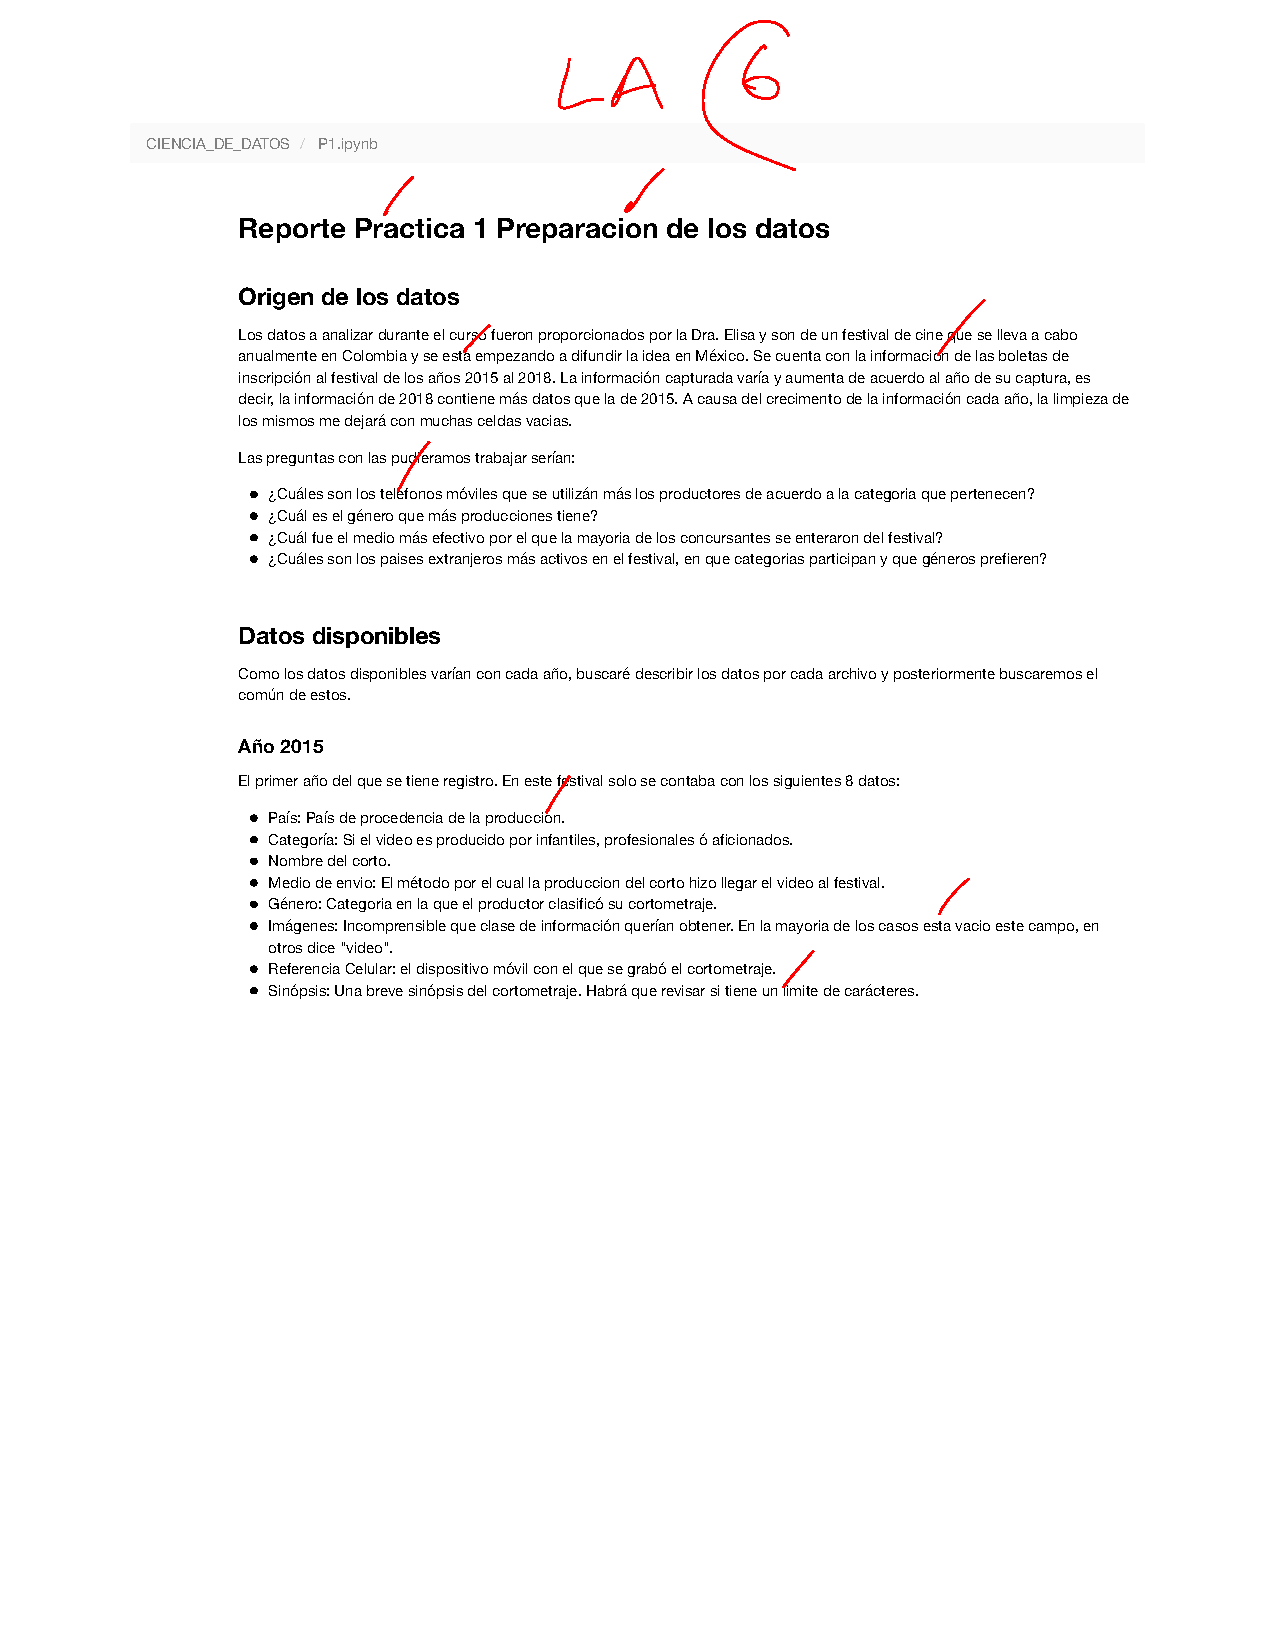
\includepdf[ pages=-, frame, scale=.85]{LA1}
\section*{Comentarios}
Durante la primera práctica, no sentí que la materia estuviera difícil. Me pareció entretenido ver los datos y pensaba en que cosas podría encontrar. En esta actividad obtuve un $6/7$ por mis errores de ortografía.

Fue interesante trabajar con los archivos desde consola sin tener que abrir un programa. Para mí fue algo nuevo utilizar los comandos bash para ver el contenido de un archivo que no fuera bloc de notas. Además pude hacer filtrado de información desde consola.

Jamás llegué a pensar que trataría con una cantidad considerable de datos, sin utilizar los filtros de Excel. Antes había utilizado pandas para la clase de Diseño de Experimentos, pero en esta materia aproveché más sus bondades.
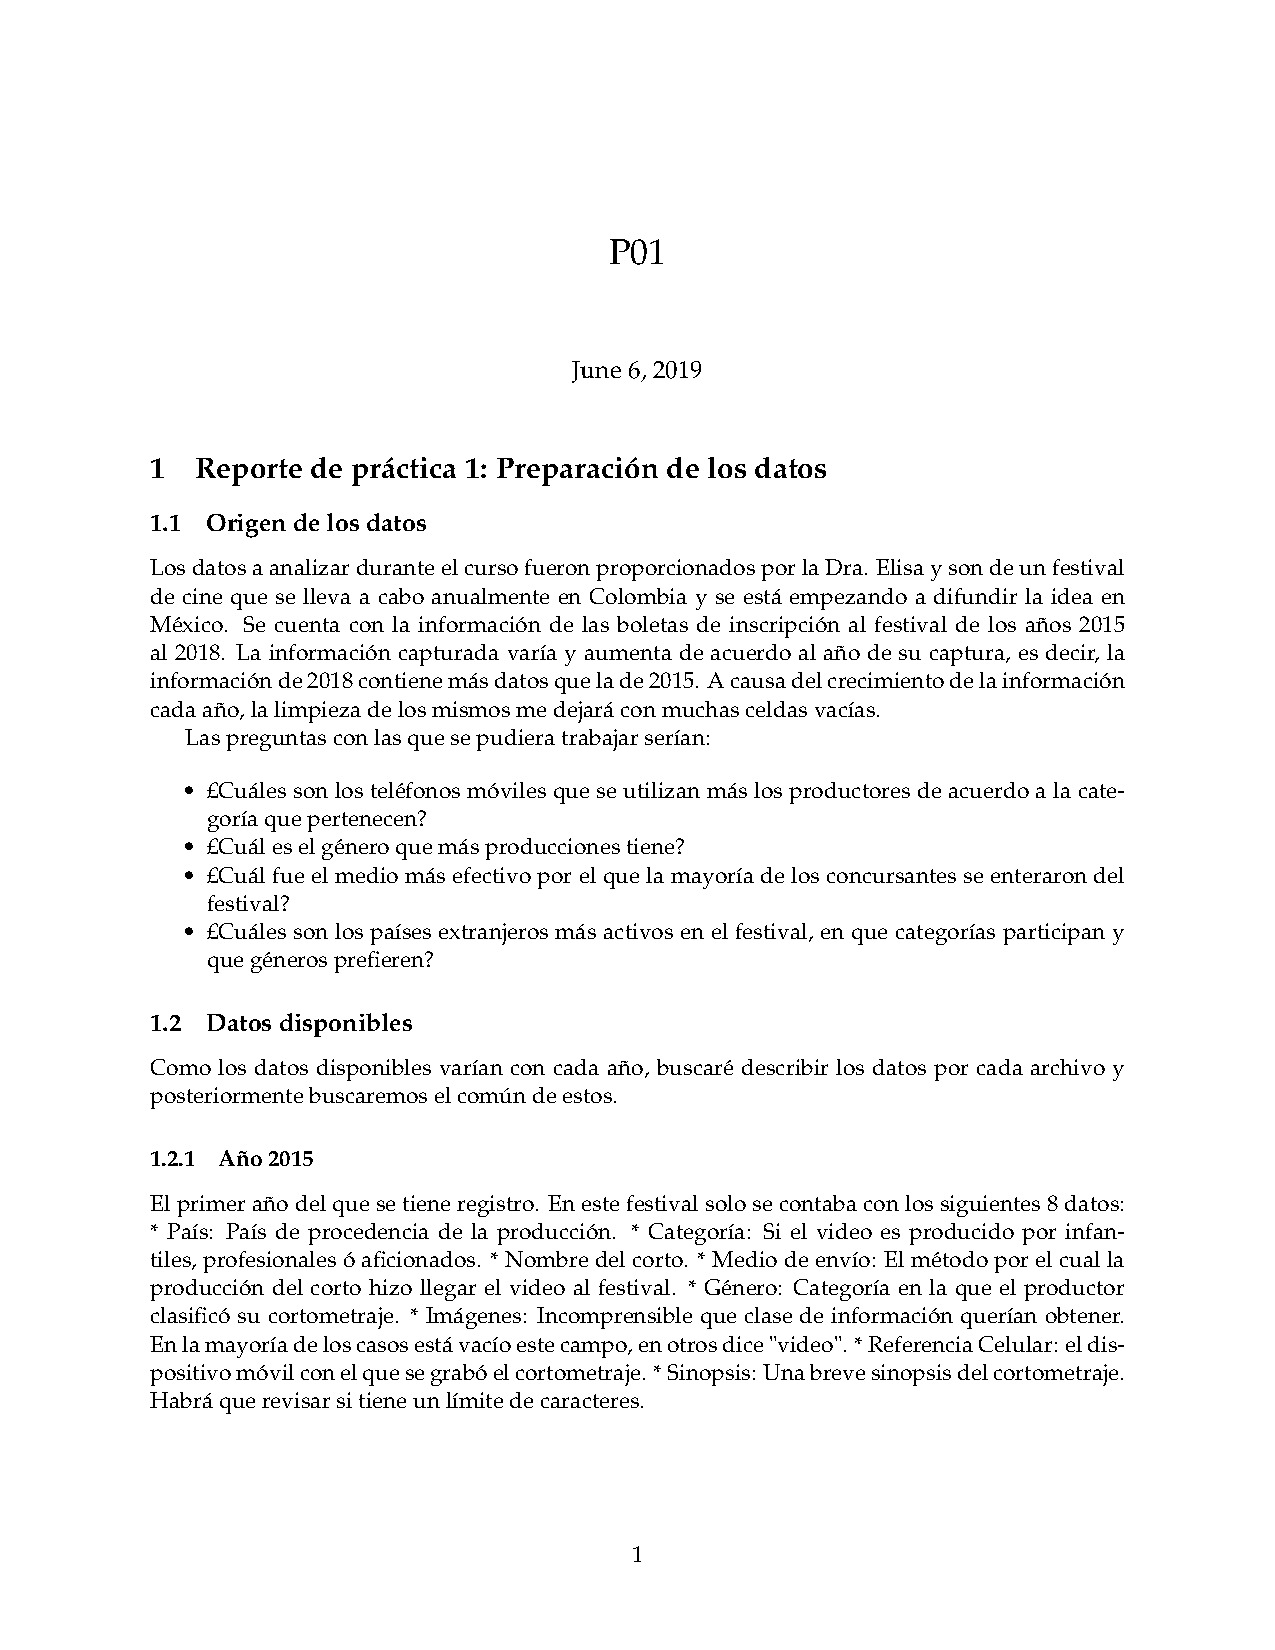
\includepdf[ pages=-, frame, scale=.85]{P01}


\chapter*{Práctica 2: Lectura y manipulación de datos}
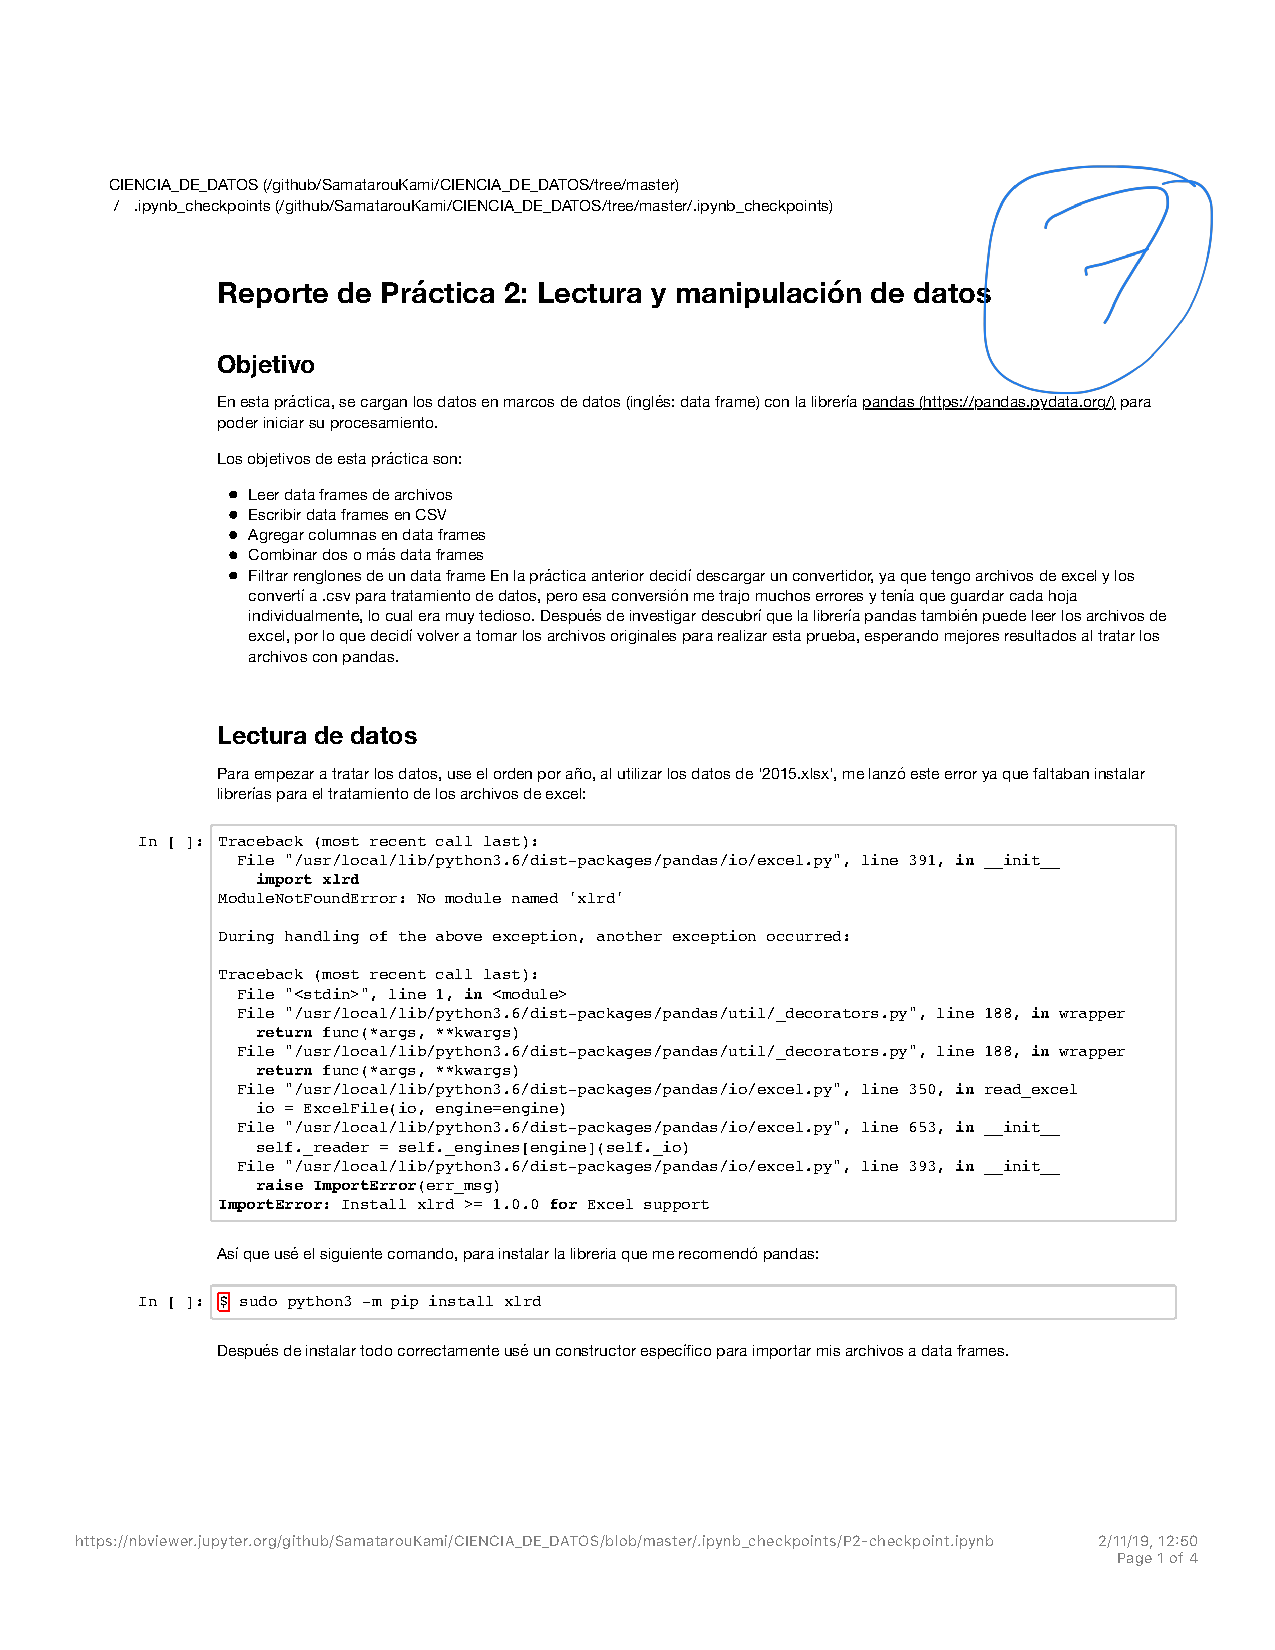
\includepdf[ pages=-, frame, scale=.85]{LA2}
\section*{Comentarios}
En esta actividad obtuve un $7/7$, no tuve complicaciones. Entendí perfectamente lo que me pedían y así lo realicé.

Lo interesante de esta práctica fue que tuve que instalar \textit{xlrd} para poder abrir los archivos con extensión de Excel en pandas de Python.
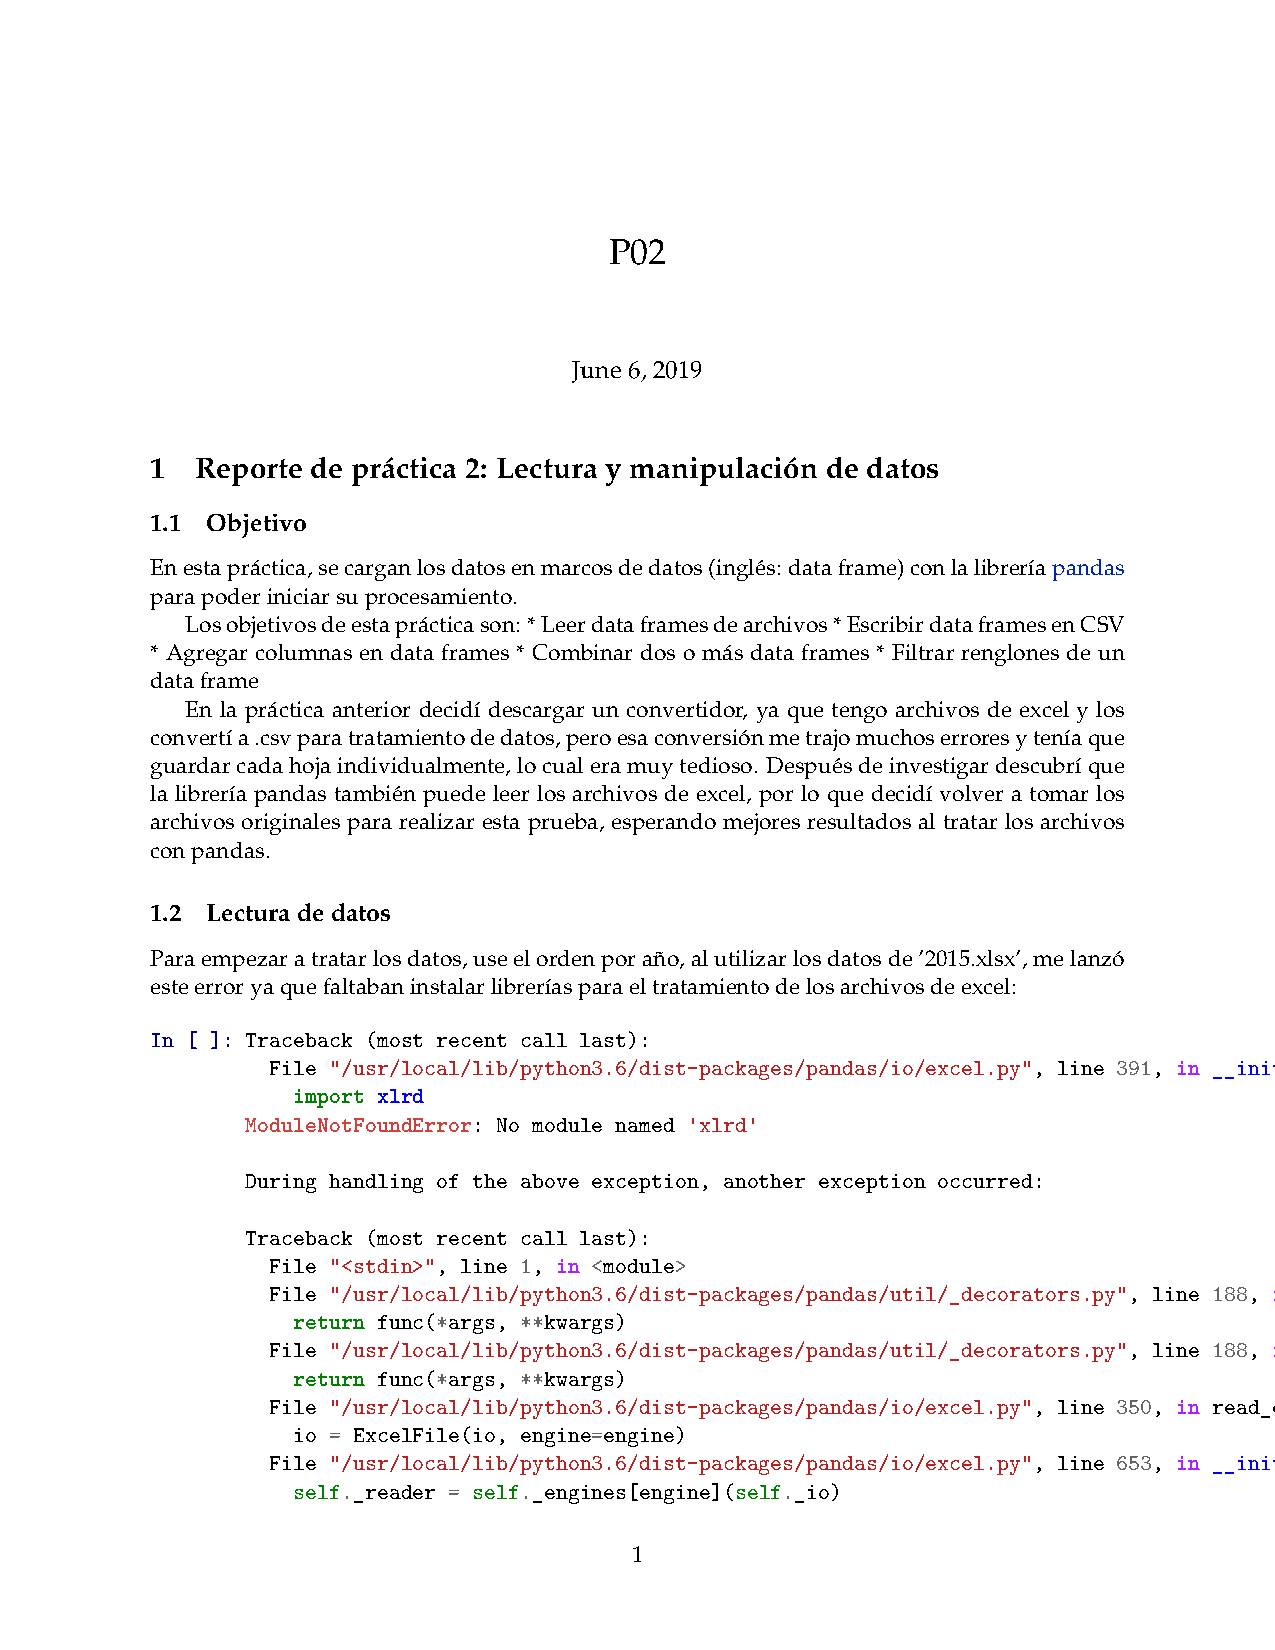
\includepdf[ pages=-, frame, scale=.85]{P02}

\chapter*{Práctica 3: Estadística descriptiva básica}
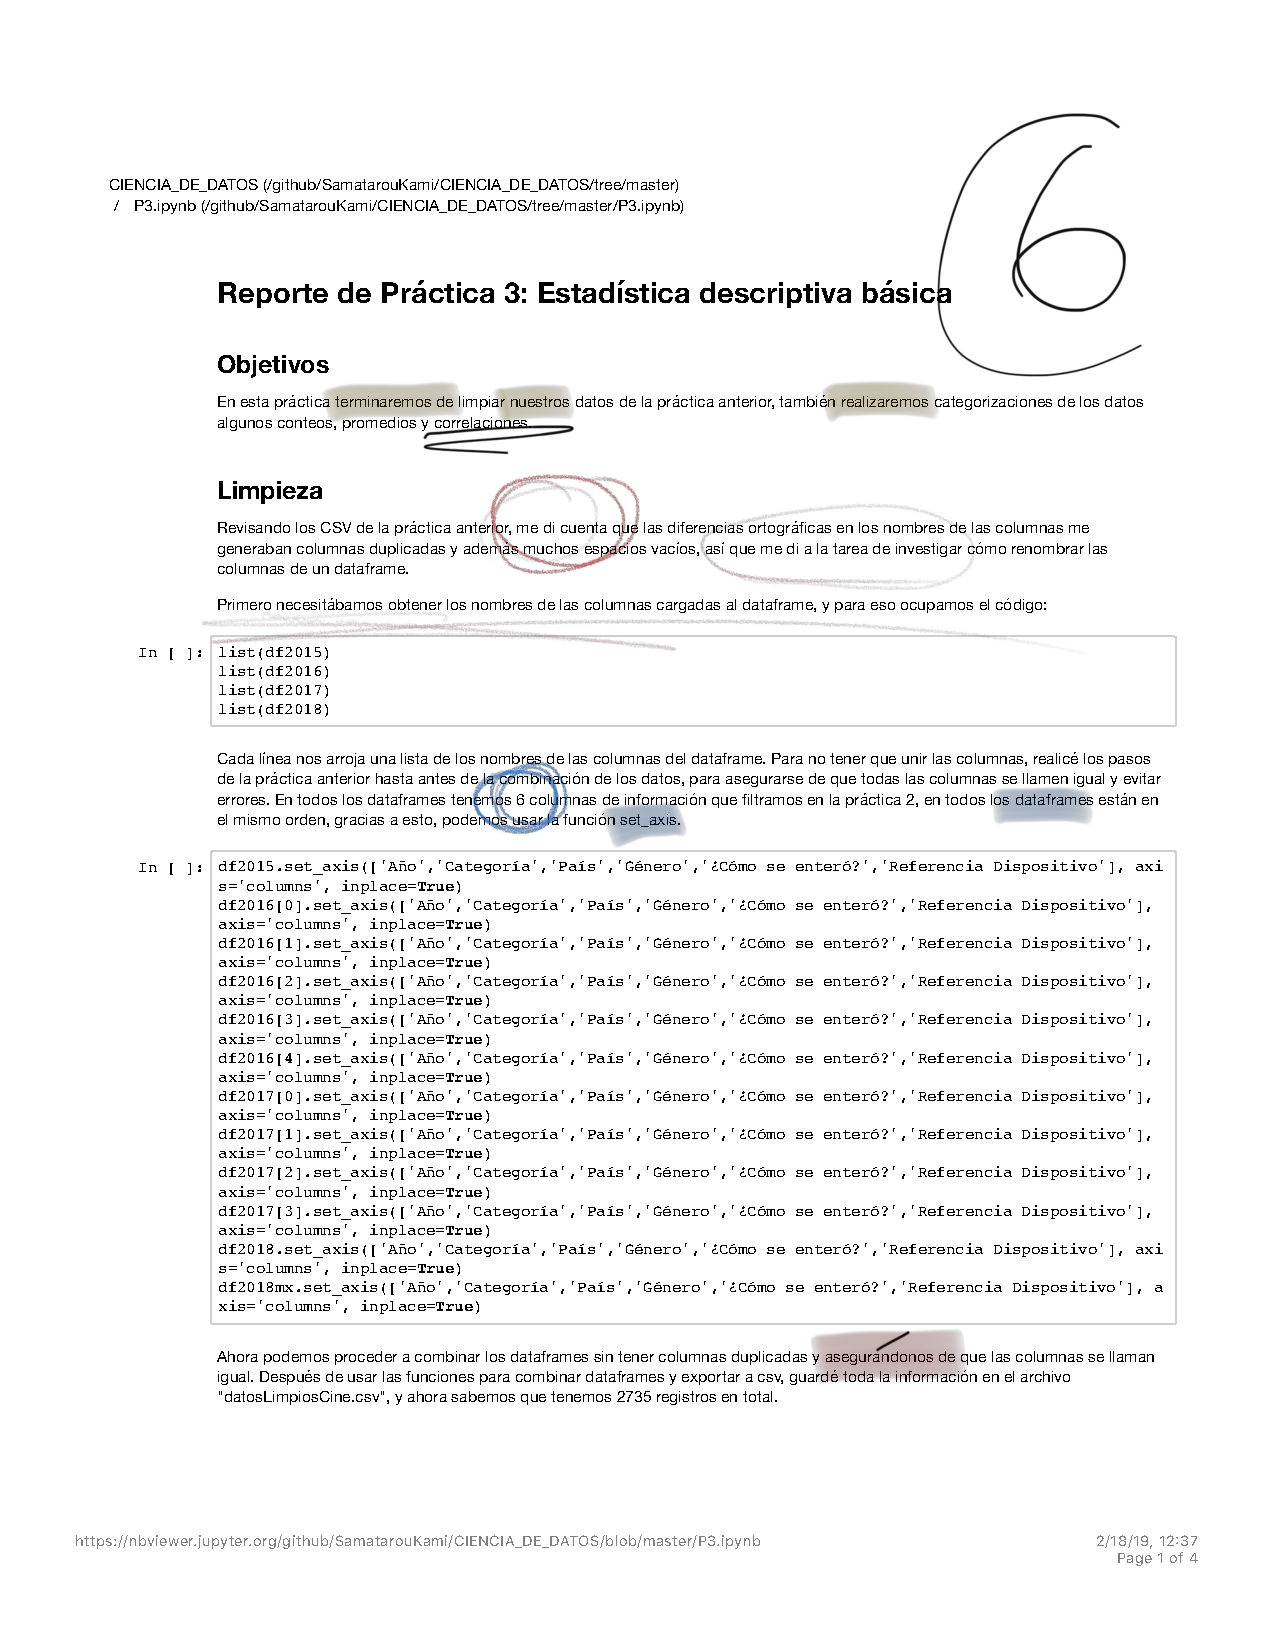
\includepdf[ pages=-, frame, scale=.85]{LA3}
\section*{Comentarios}
En esta actividad obtuve un $6/7$, principalmente por errores en la conjugación de los verbos y errores de ortografía
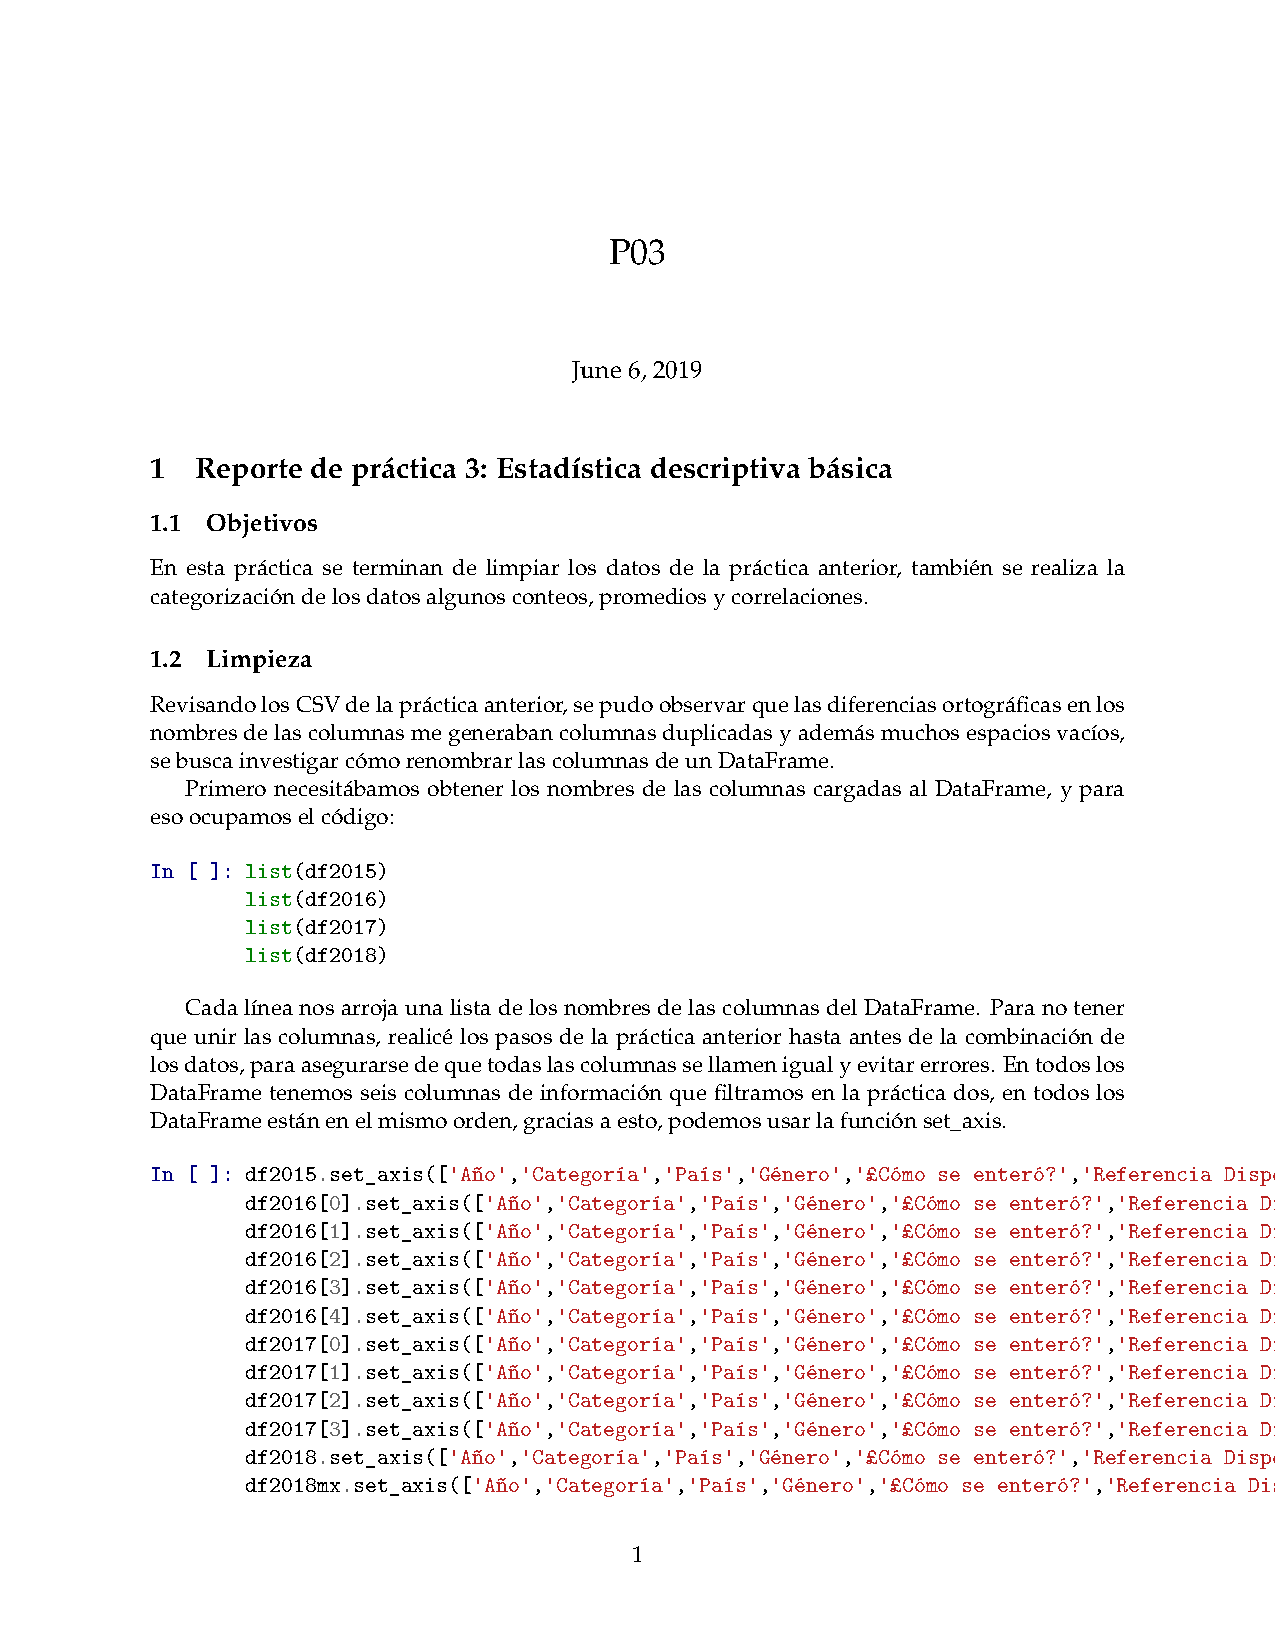
\includepdf[ pages=-, frame, scale=.85]{P03}

\chapter*{Práctica 4: Visualización de información}
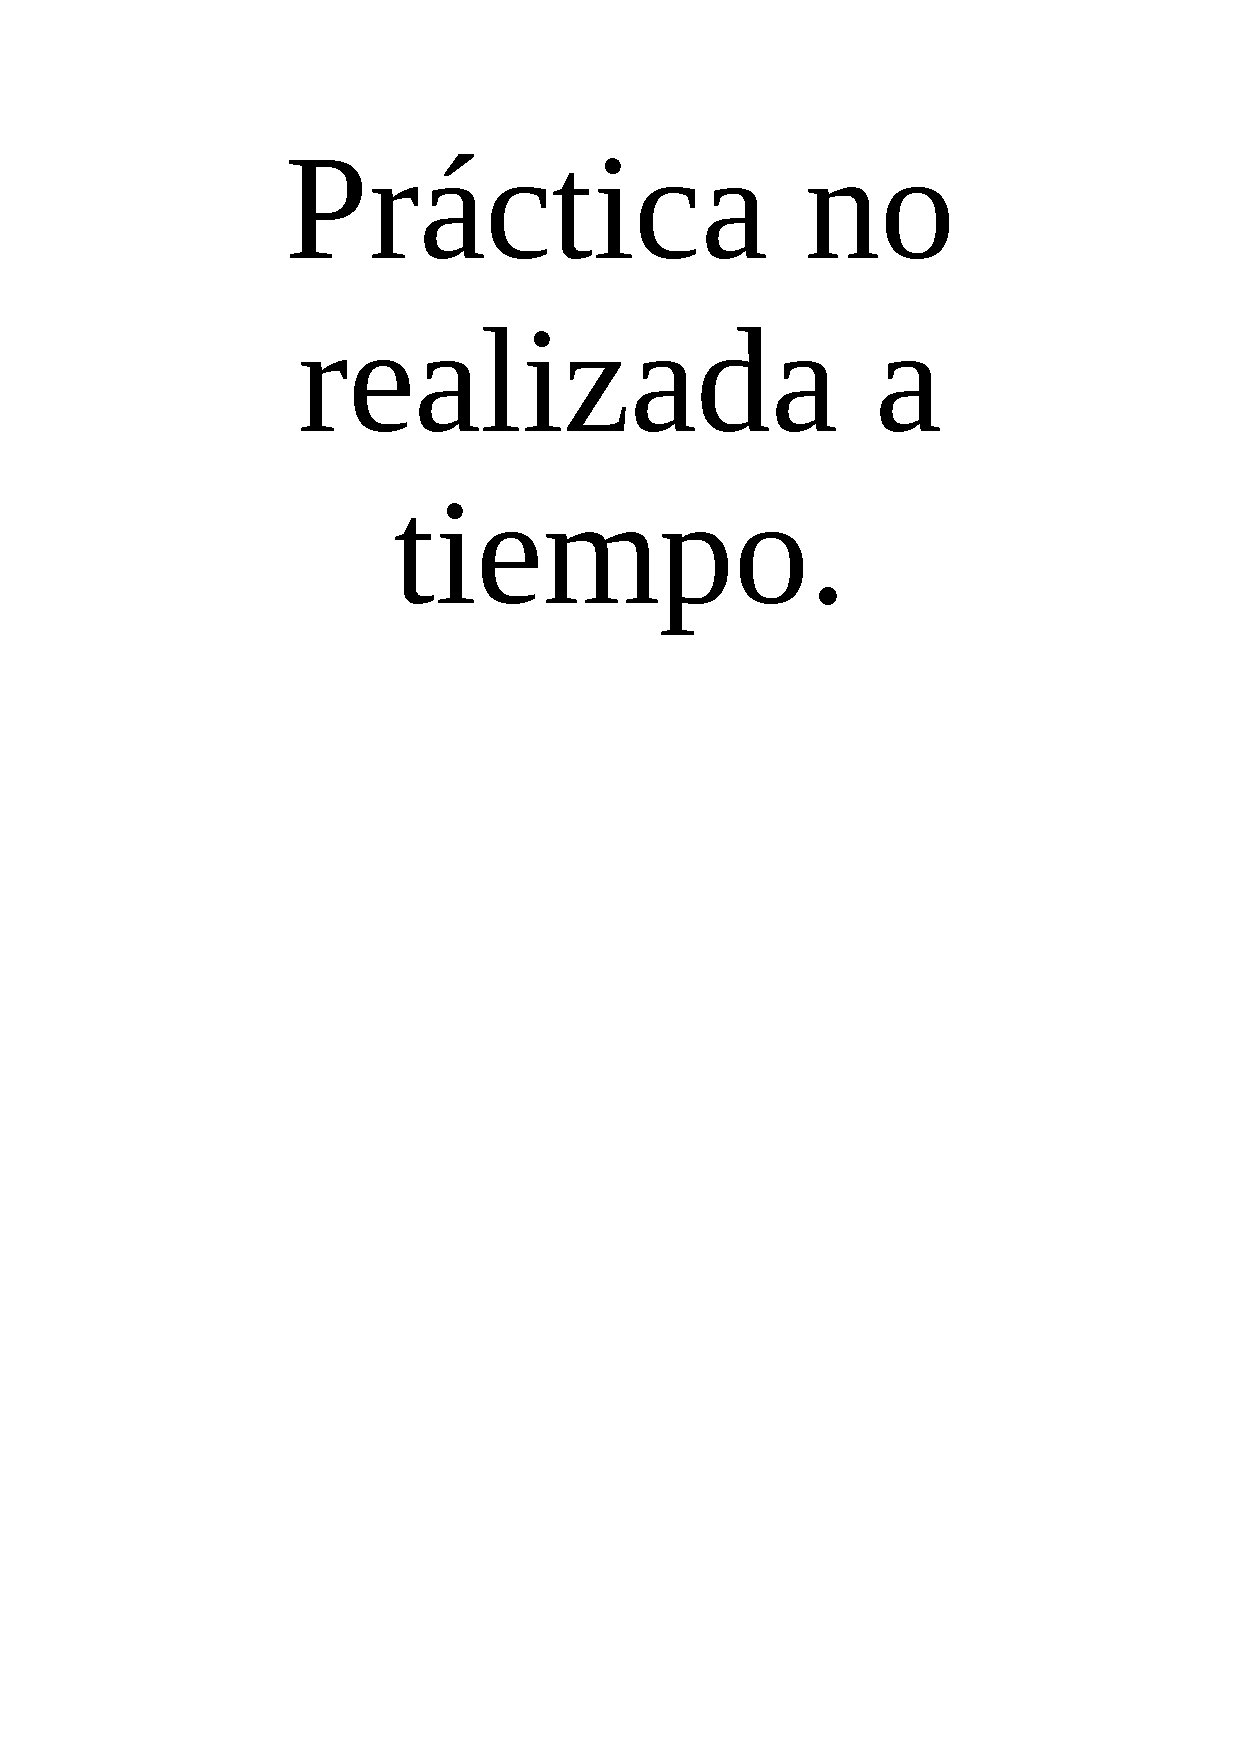
\includepdf[ pages=-, frame, scale=.85]{NP}
\section*{Comentarios}
Por no contemplar bien los tiempos de desarrollo y el tiempo de depuración de los bugs, esta tarea se me pasó hacerla. La volví a hacer pero al momento de exportarla a pdf se perdían las gráficas, solo aparecía la dirección de la imagen. Por este motivo para poder visualizarlas, simulé que las imprimía, y salieron cortados los gráficos.
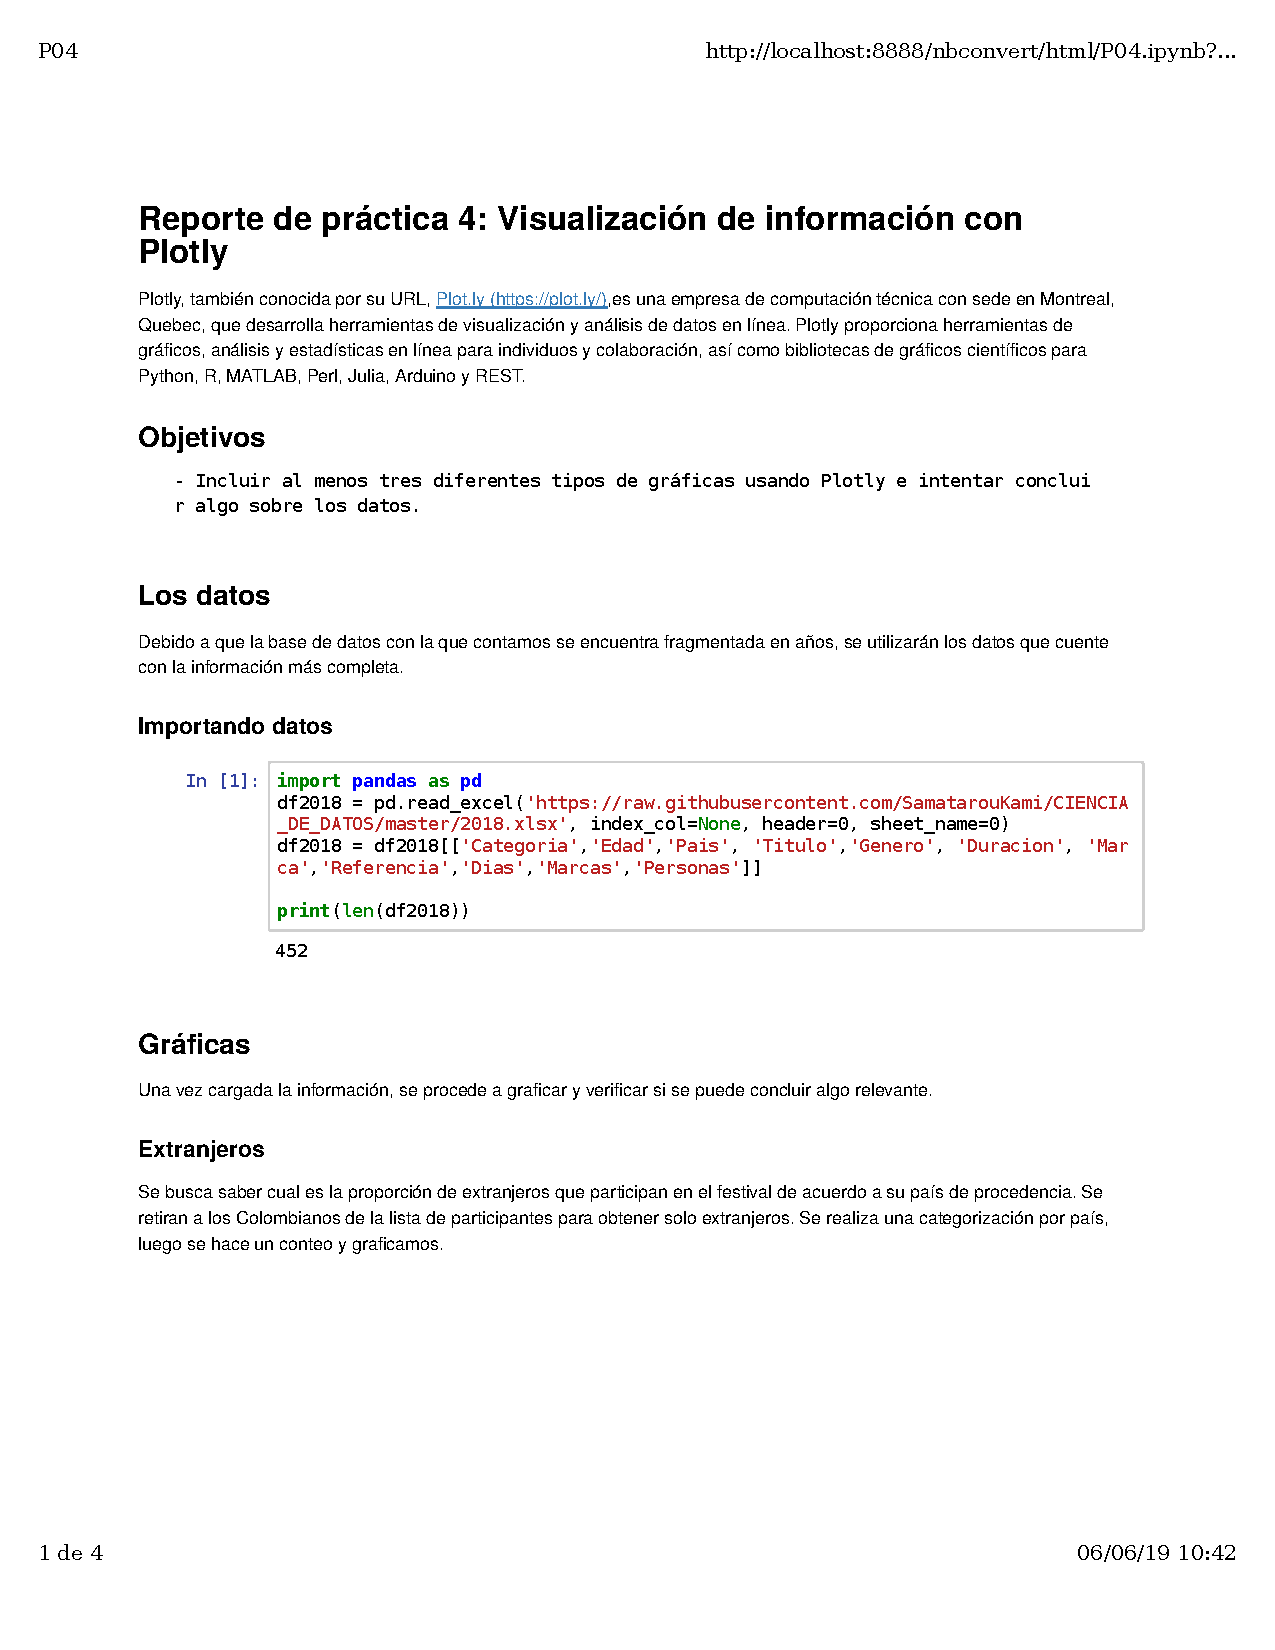
\includepdf[ pages=-, frame, scale=.85]{P04}

\chapter*{Práctica 5: Pruebas estadísticas}
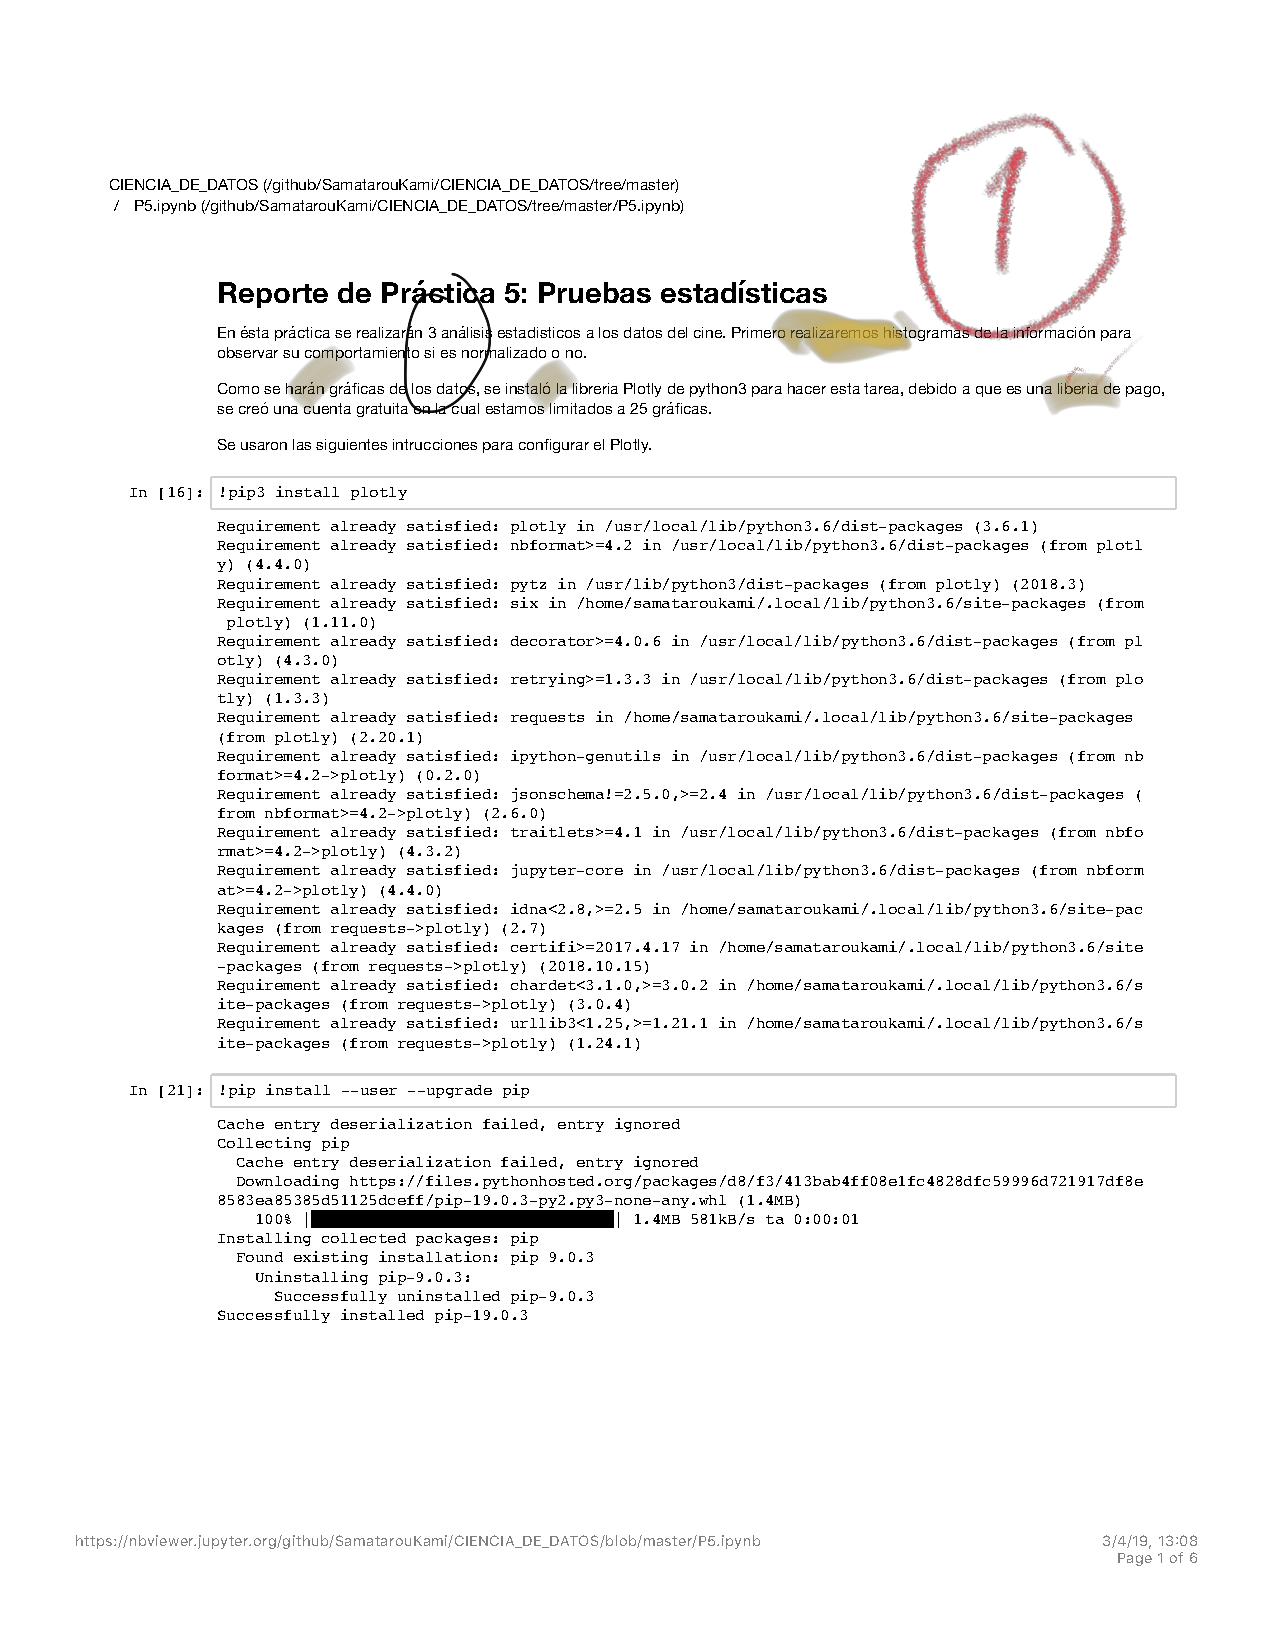
\includepdf[ pages=-, frame, scale=.85]{LA5}
\section*{Comentarios}
En esta actividad obtuve un $1/7$, el principal problema no lo pude identificar hasta dos practicas después. Tenia nombres de variables con acentos. Aquí solo pude instalar las librerías y no corrí nada, por esto mi merecido 1. Al rehacer la actividad logré completar los objetivos de la misma. Realicé las tres diferentes tipos de pruebas estadísticas de hipótesis. Y corregí los errores de ortografía que tenía. 
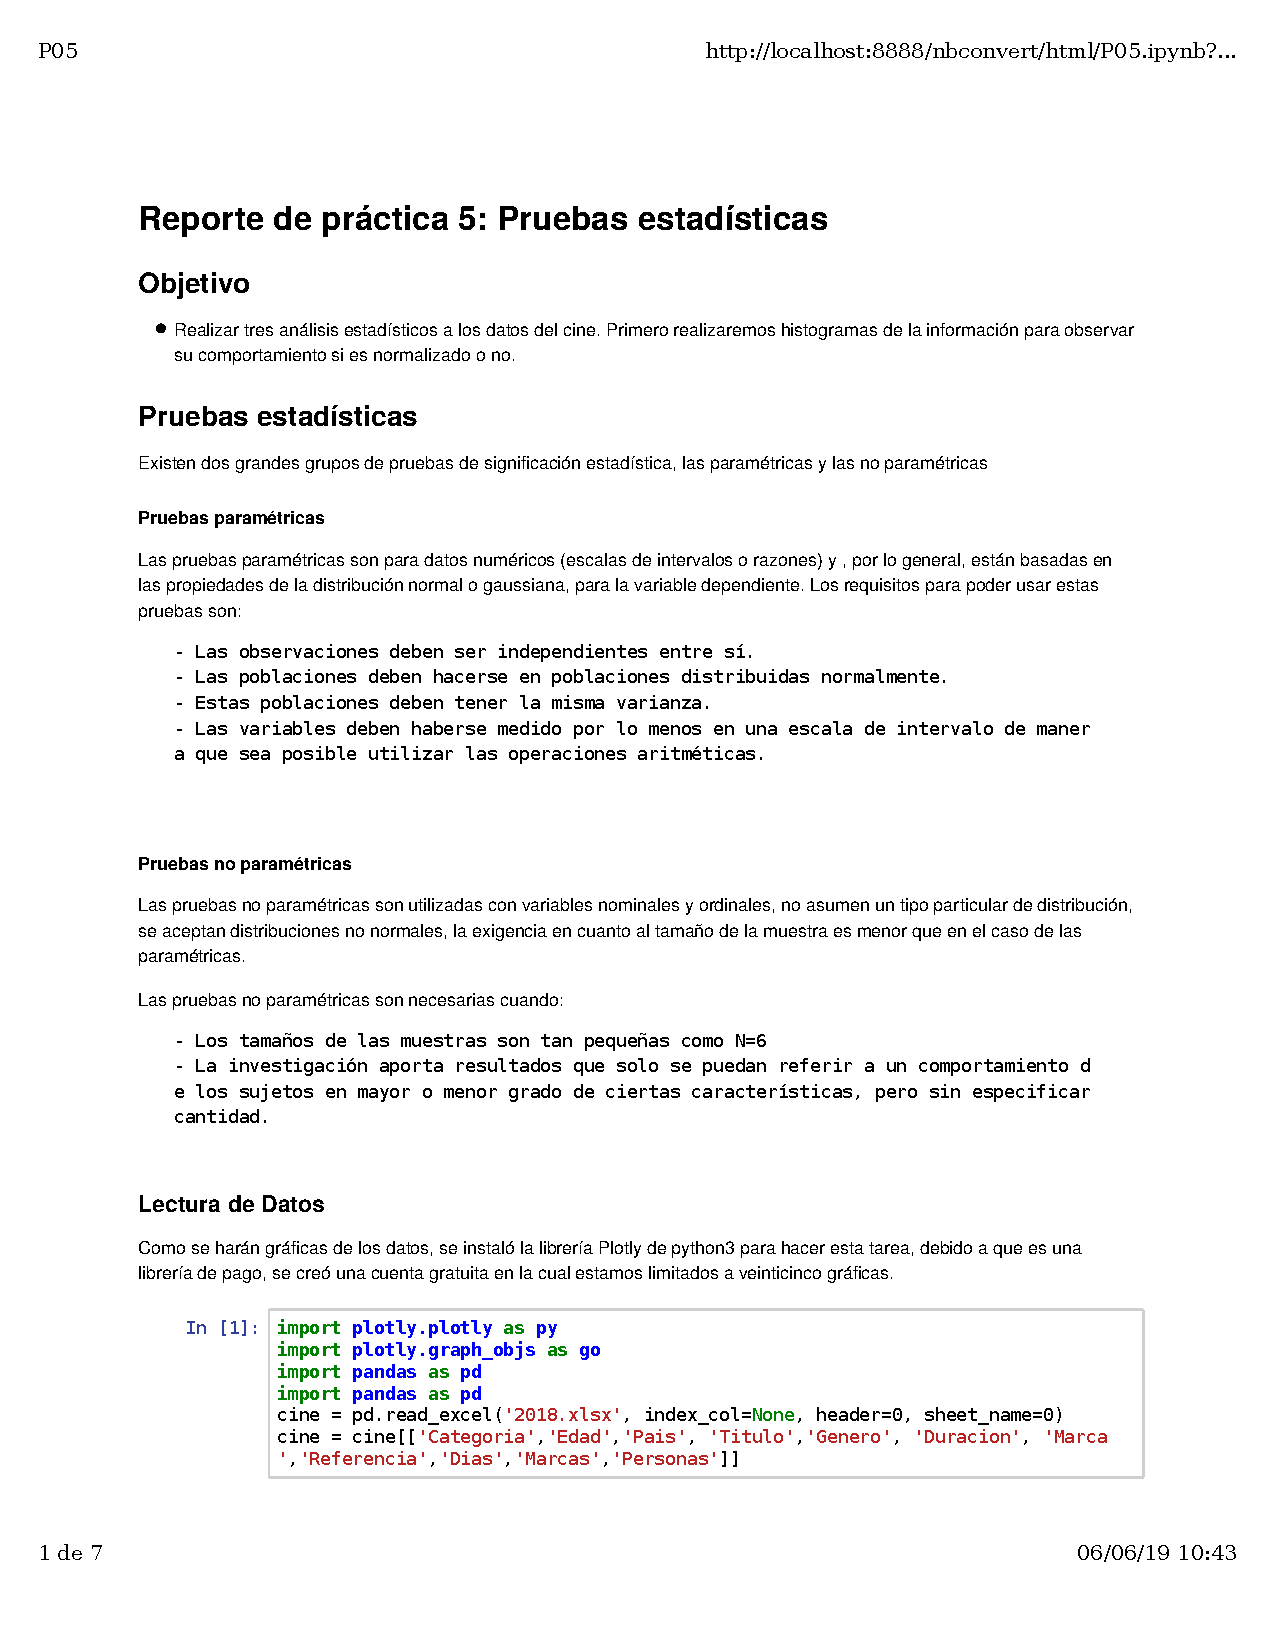
\includepdf[ pages=-, frame, scale=.85]{P05}

\chapter*{Práctica 6: Modelos lineales}
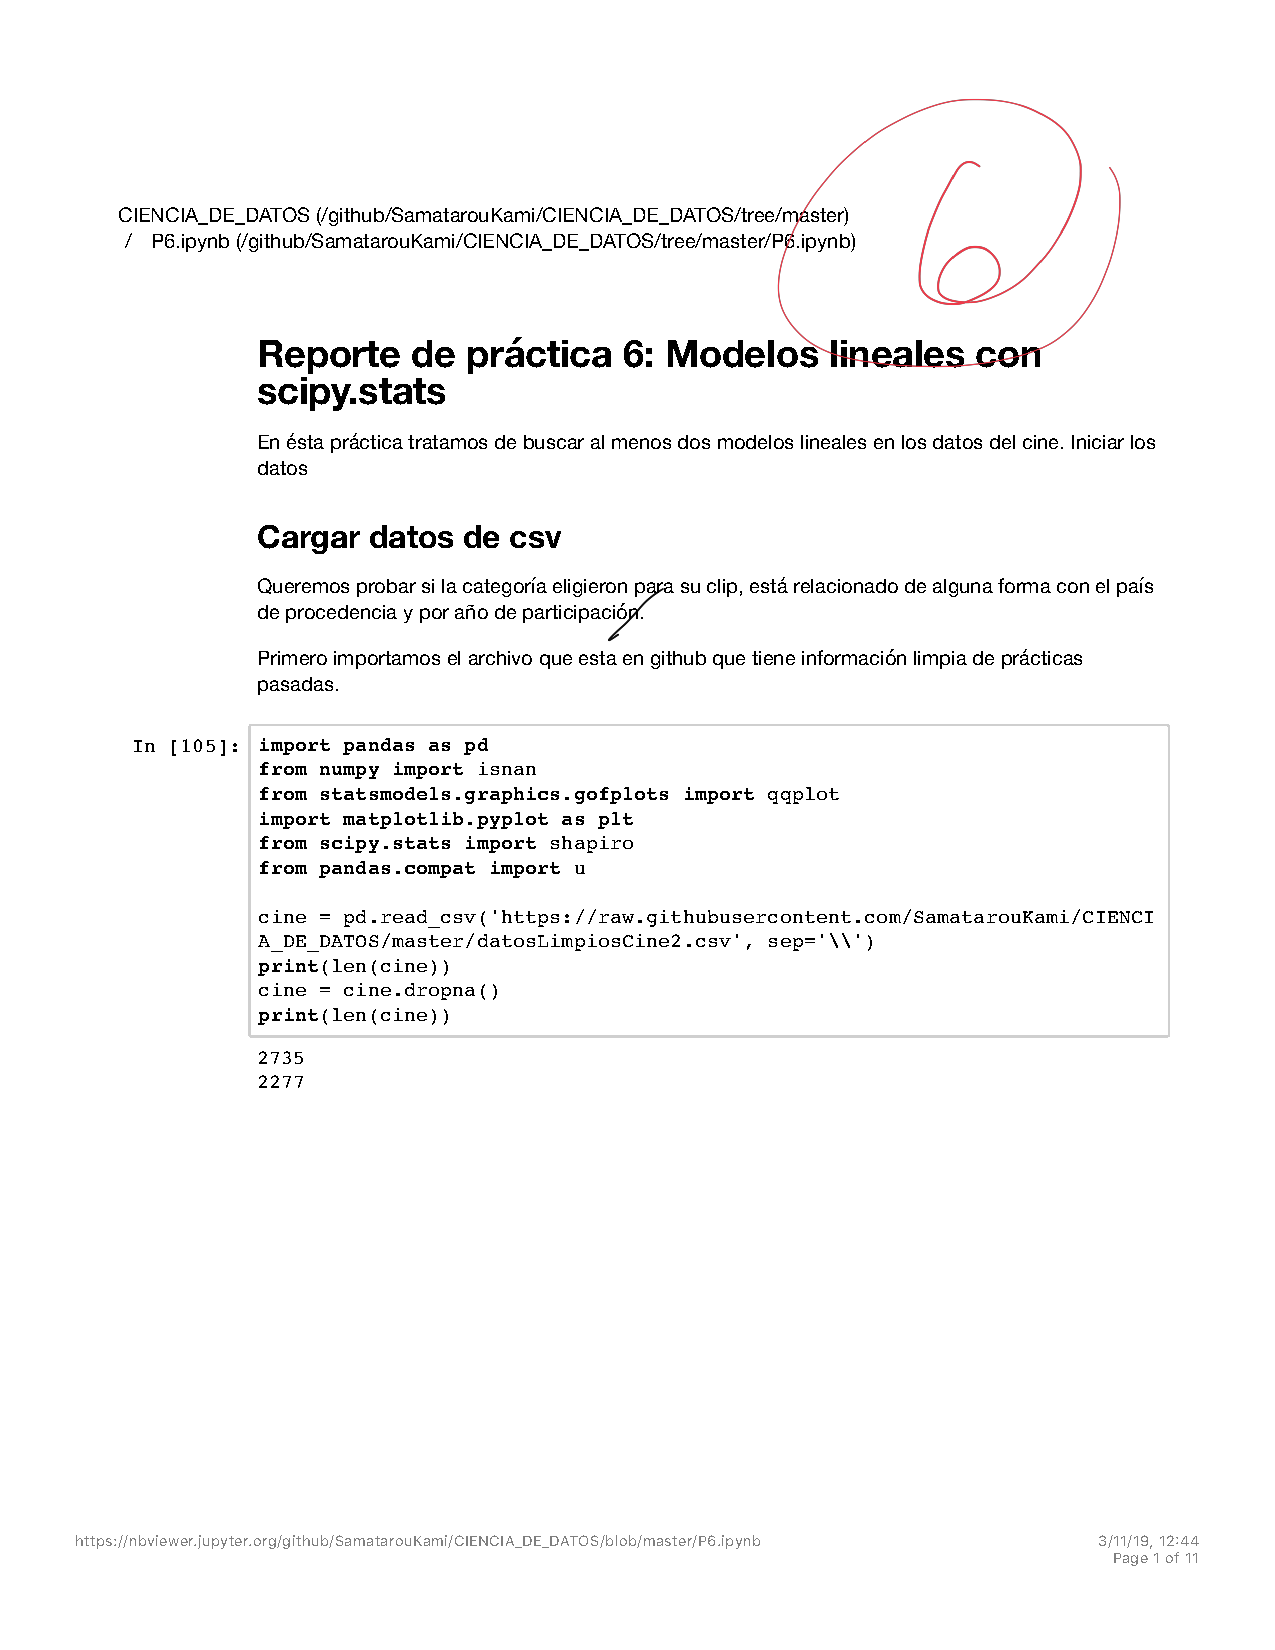
\includepdf[ pages=-, frame, scale=.85]{LA6}
\section*{Comentarios}
En esta actividad obtuve un $6/7$, esta práctica la entendí muy bien. El punto que perdí fue por la ortografía nuevamente. 
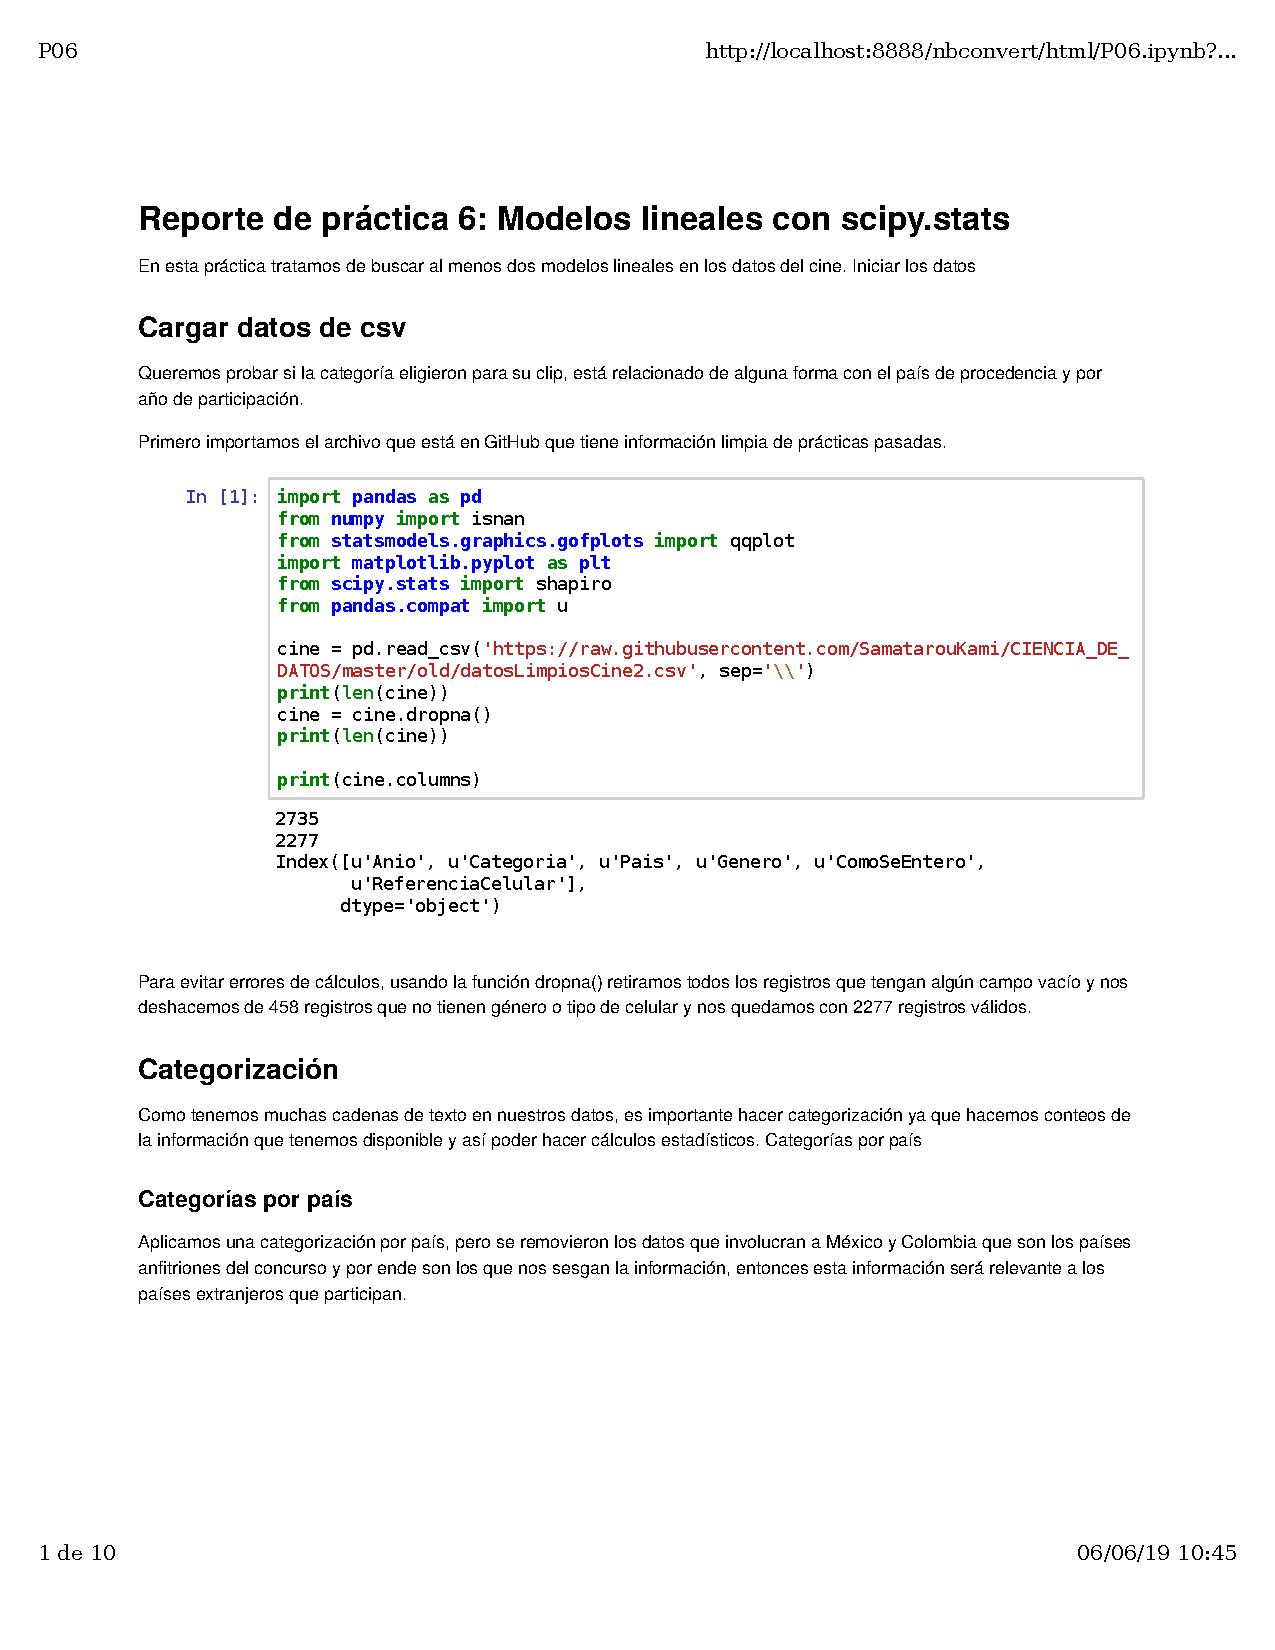
\includepdf[ pages=-, frame, scale=.85]{P06}

\chapter*{Práctica 7: Regresión múltiple}
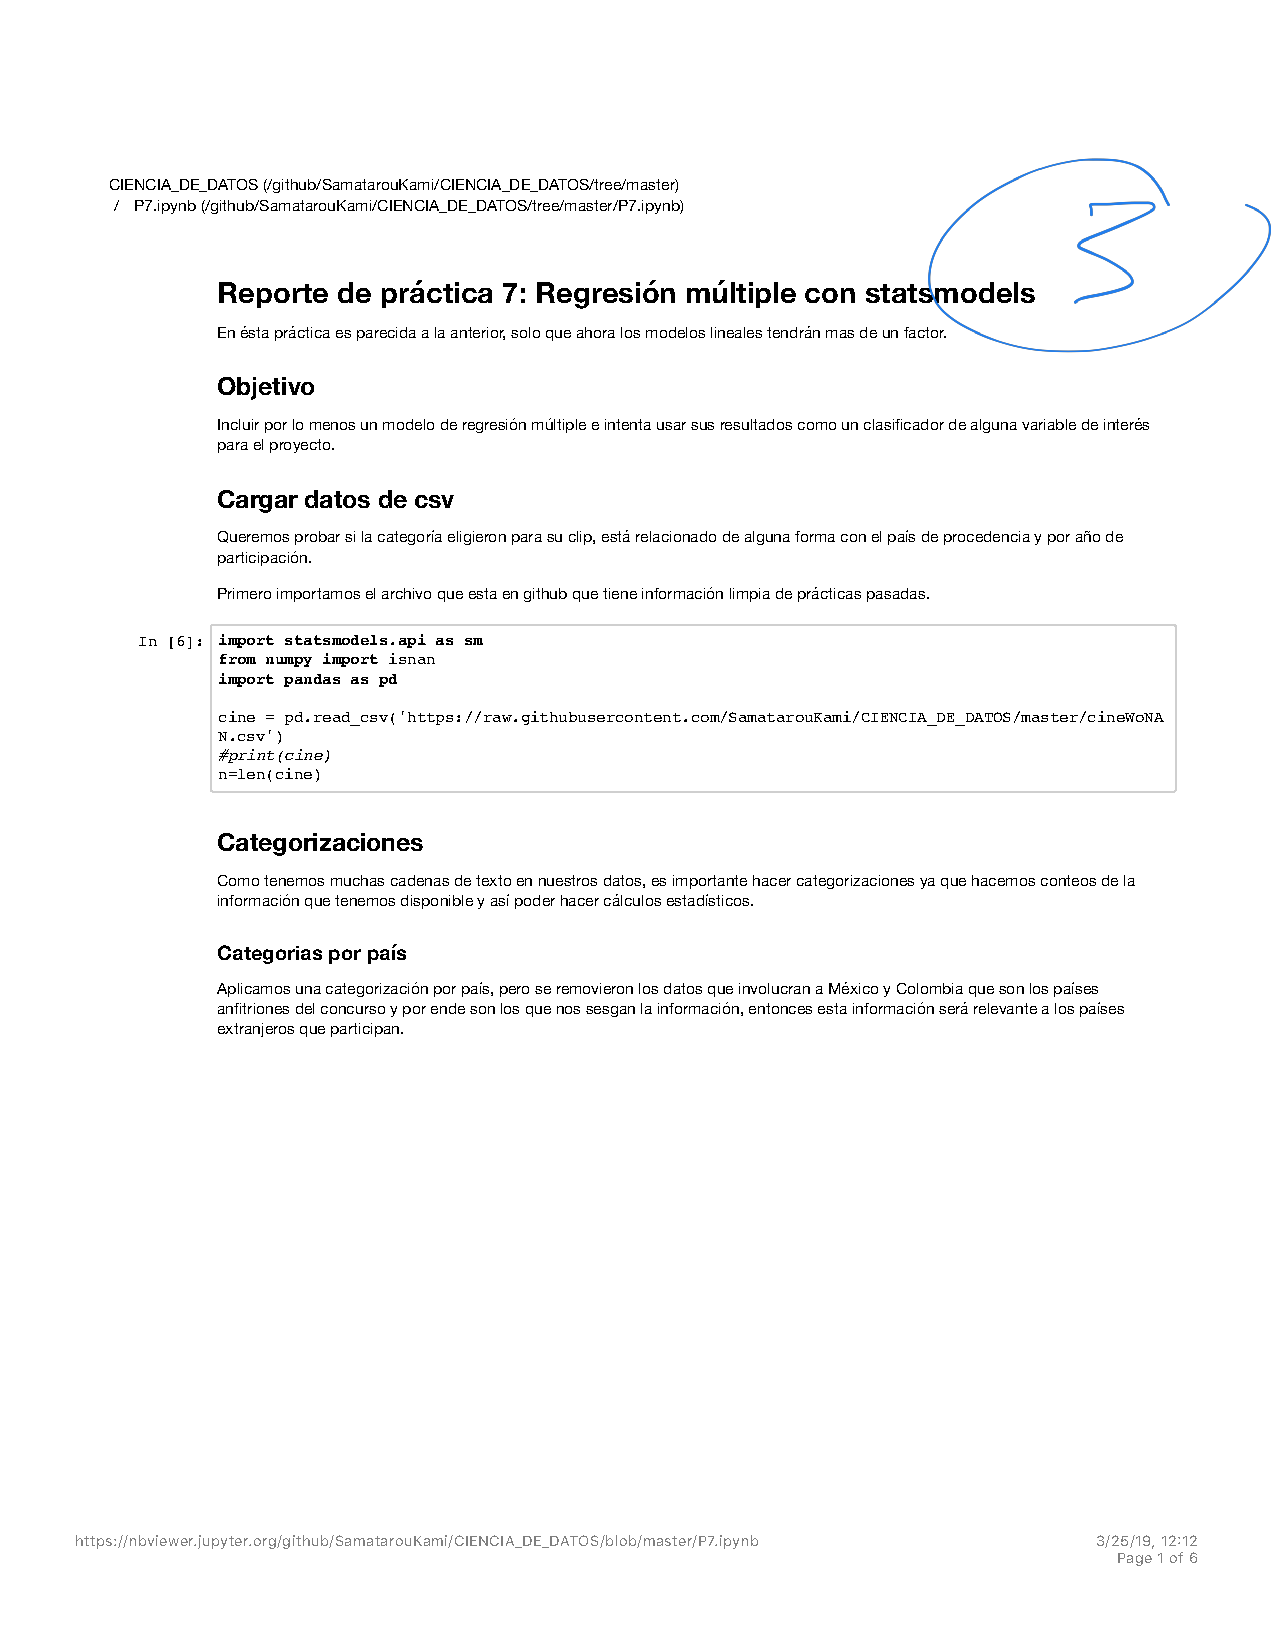
\includepdf[ pages=-, frame, scale=.85]{LA7}
\section*{Comentarios}
En esta actividad obtuve un $3/7$ porque además de que mi prueba de hipótesis era súper fácil, ya que todos los valores estaban fuertemente correlacionado. Se me olvidó realizar un pronostico basándonos en la función que generó el OLS.
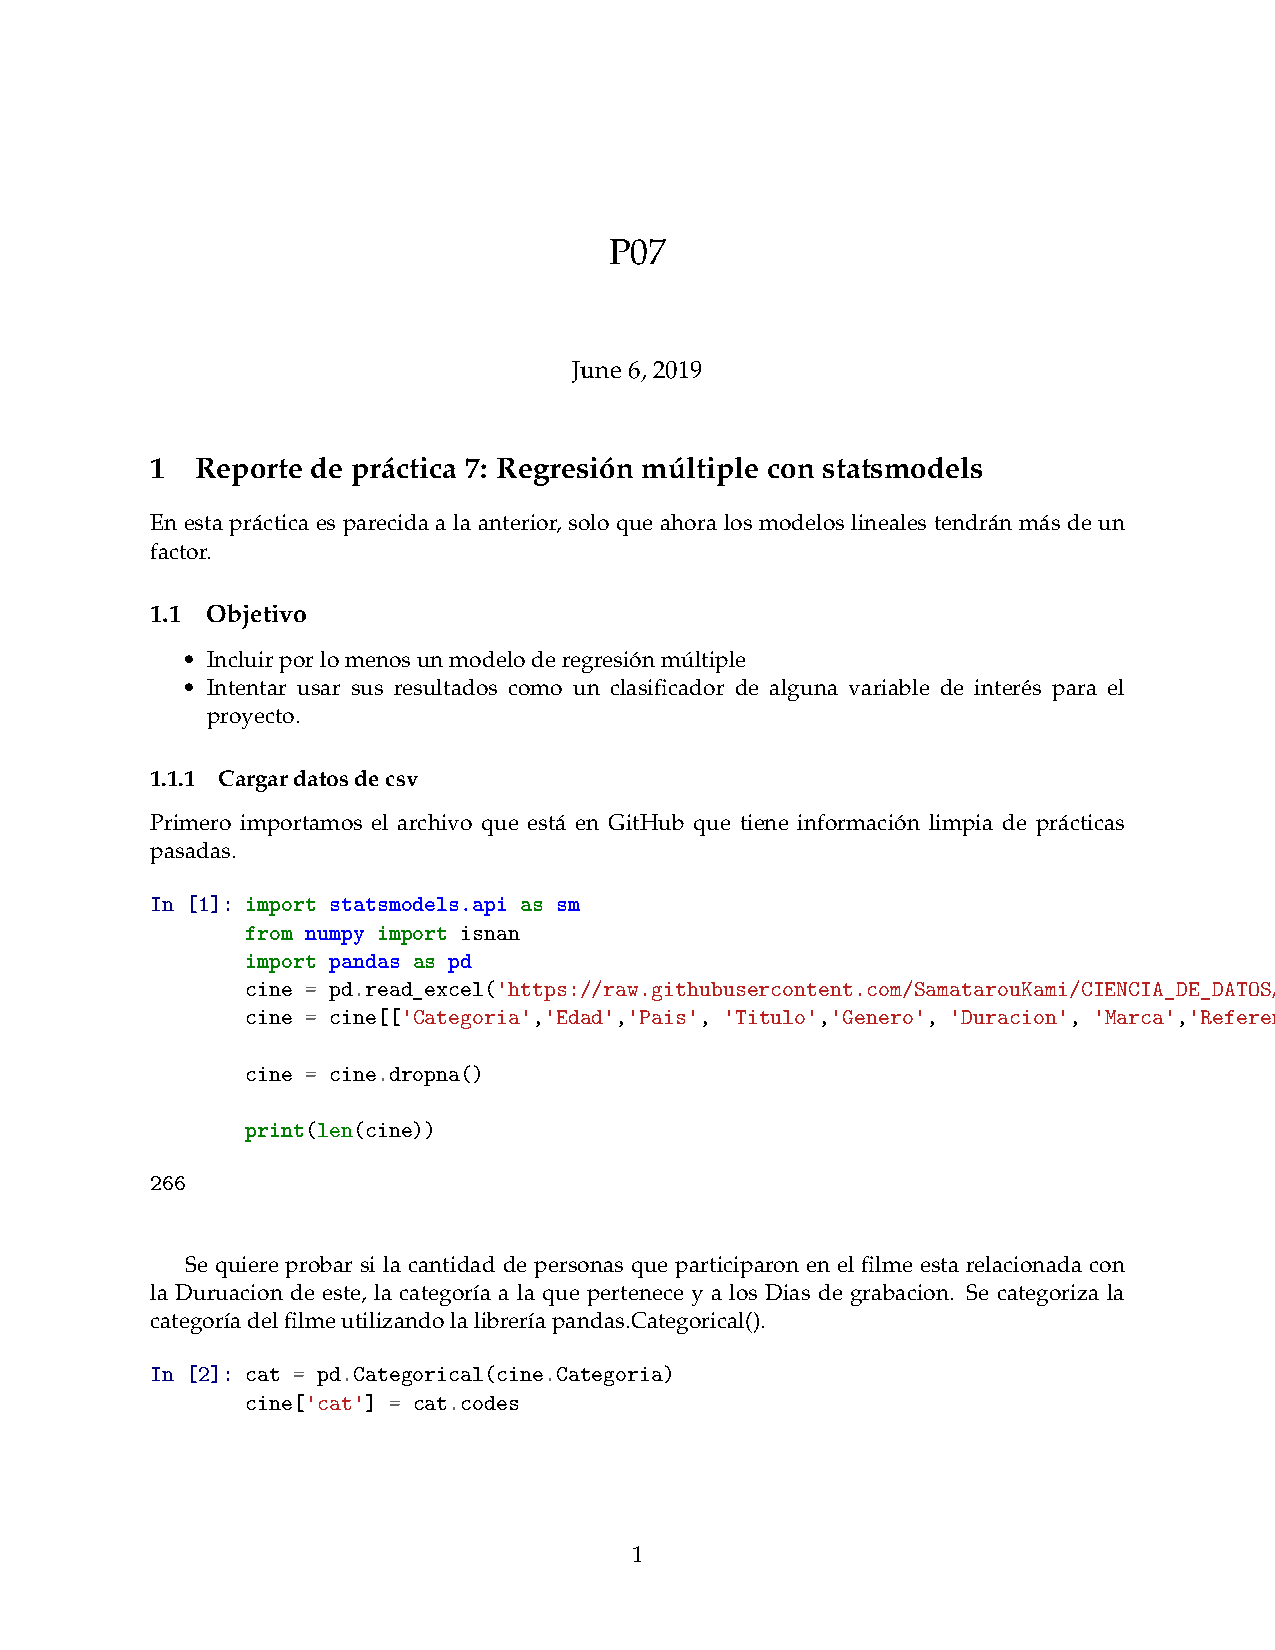
\includepdf[ pages=-, frame, scale=.85]{P07}

\chapter*{Práctica 8: Análisis de varianza y de componentes principales}
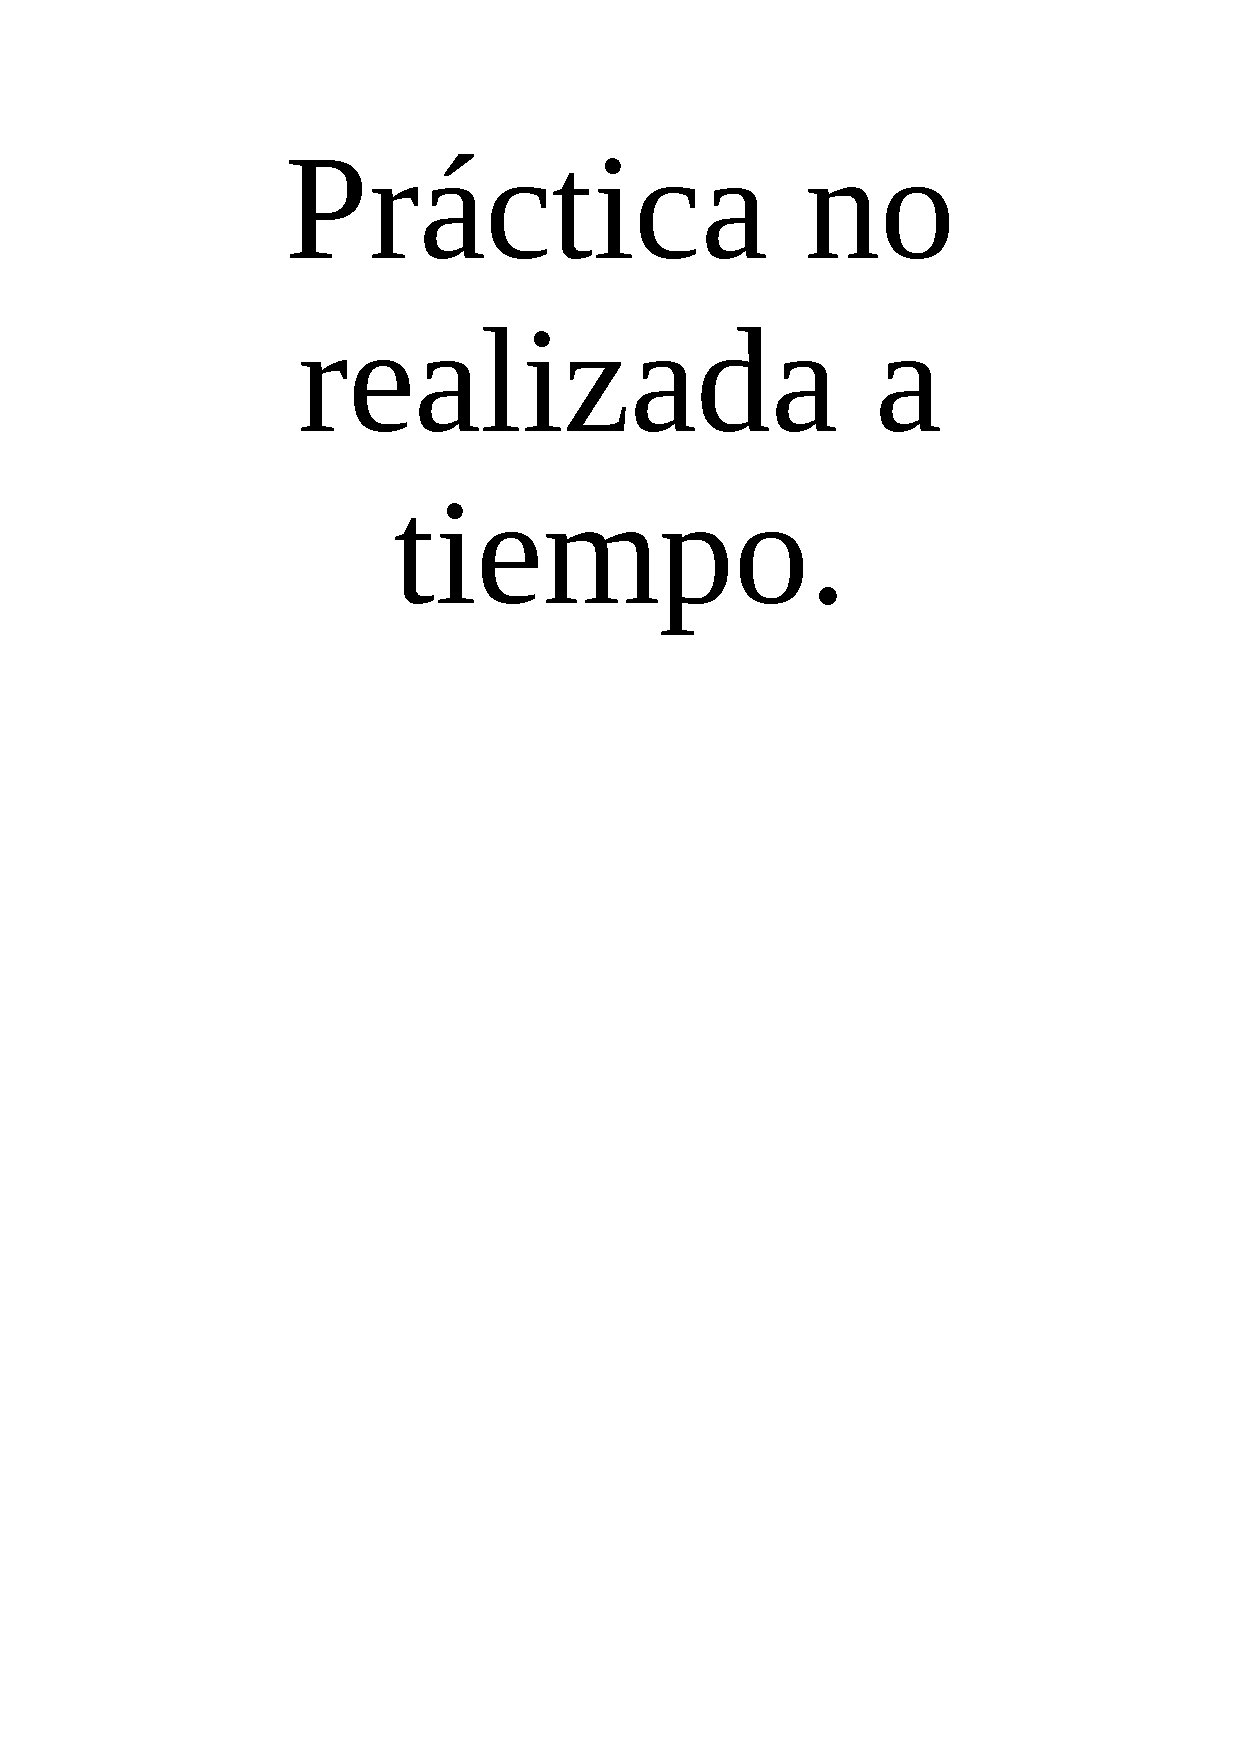
\includepdf[ pages=-, frame, scale=.85]{NP}
\section*{Comentarios}
Por no contemplar bien los tiempos de desarrollo y el tiempo de depuración de los bugs, esta tarea no pude hacerla. Cuando me dí el tiempo para hacerla y entregarla en este portafolio, pude hacer el ANOVA y el PCA. En el ANOVA, habían tres variables que eran significativas, pero al momento de buscar si cuando interactúan seguían siendo significativas no lo eran.
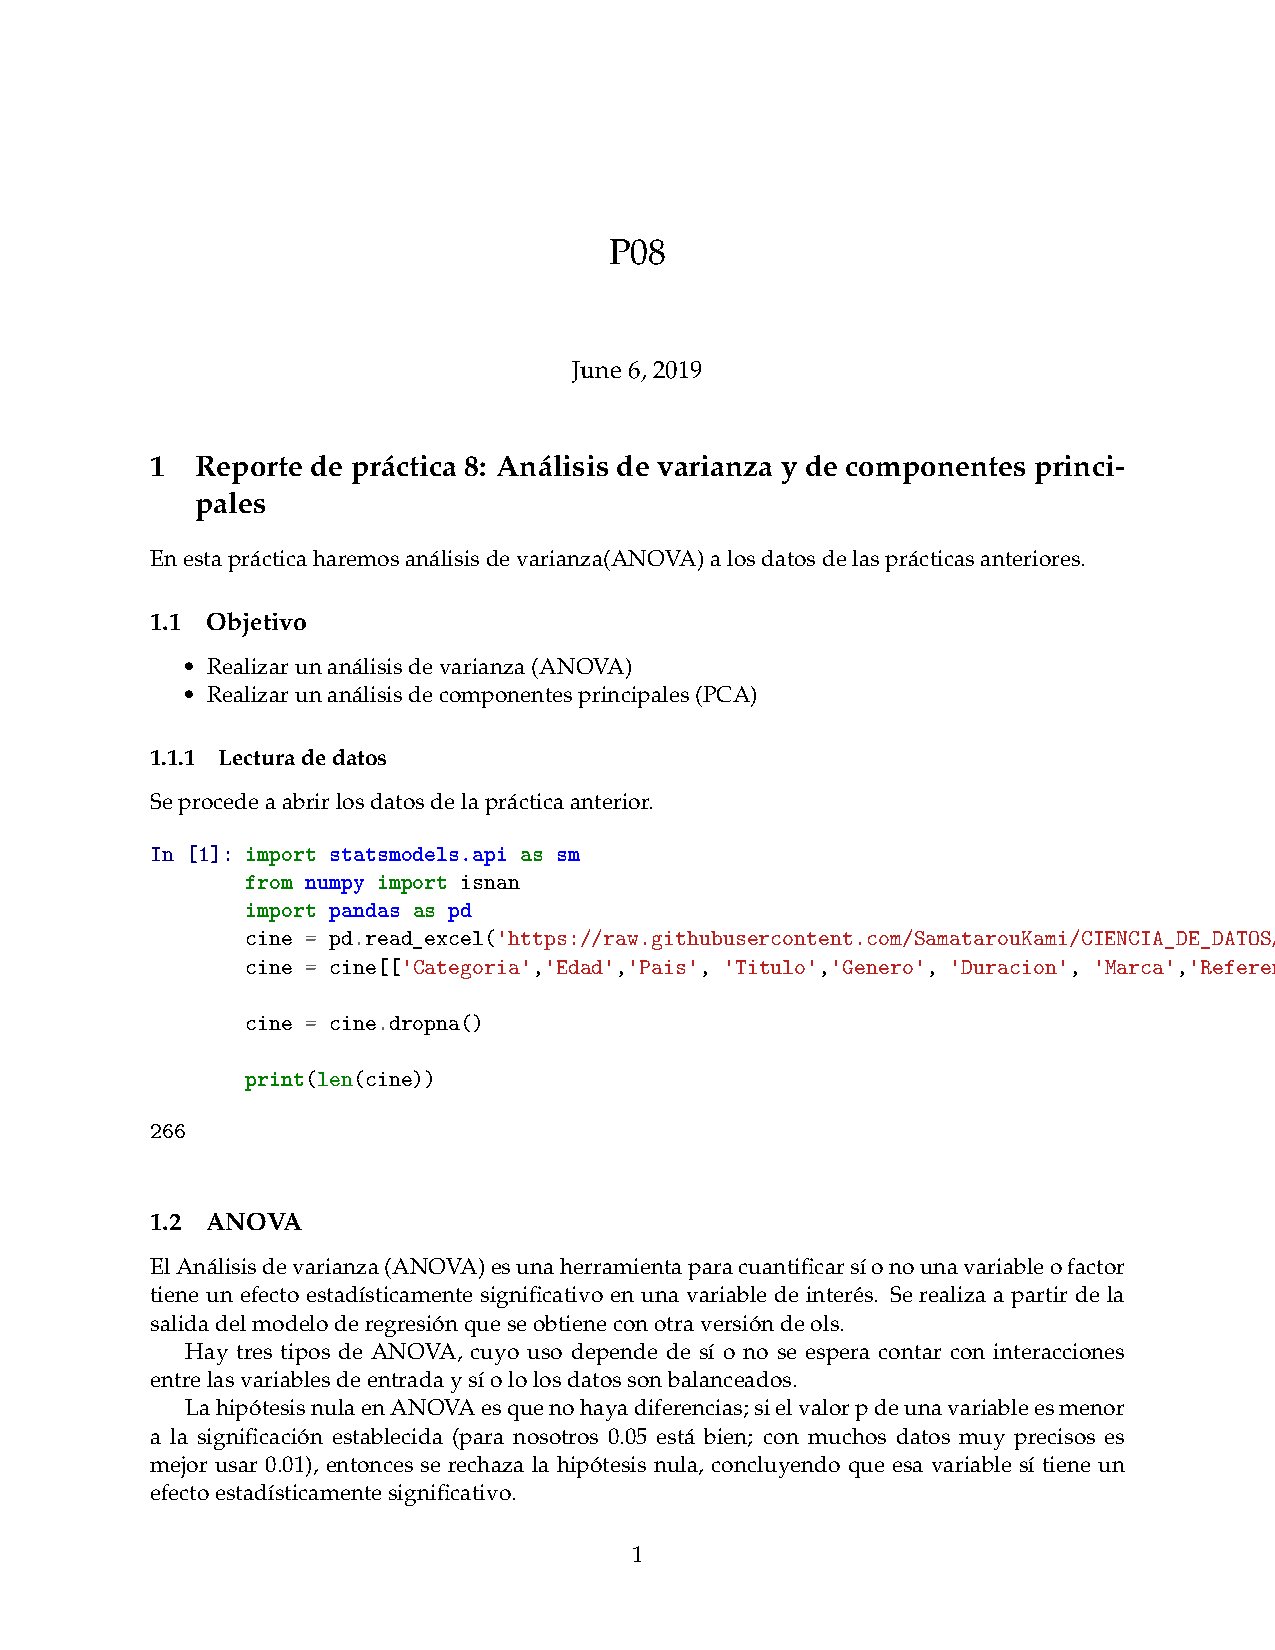
\includepdf[ pages=-, frame, scale=.85]{P08}

\chapter*{Práctica 9: Pronósticos}
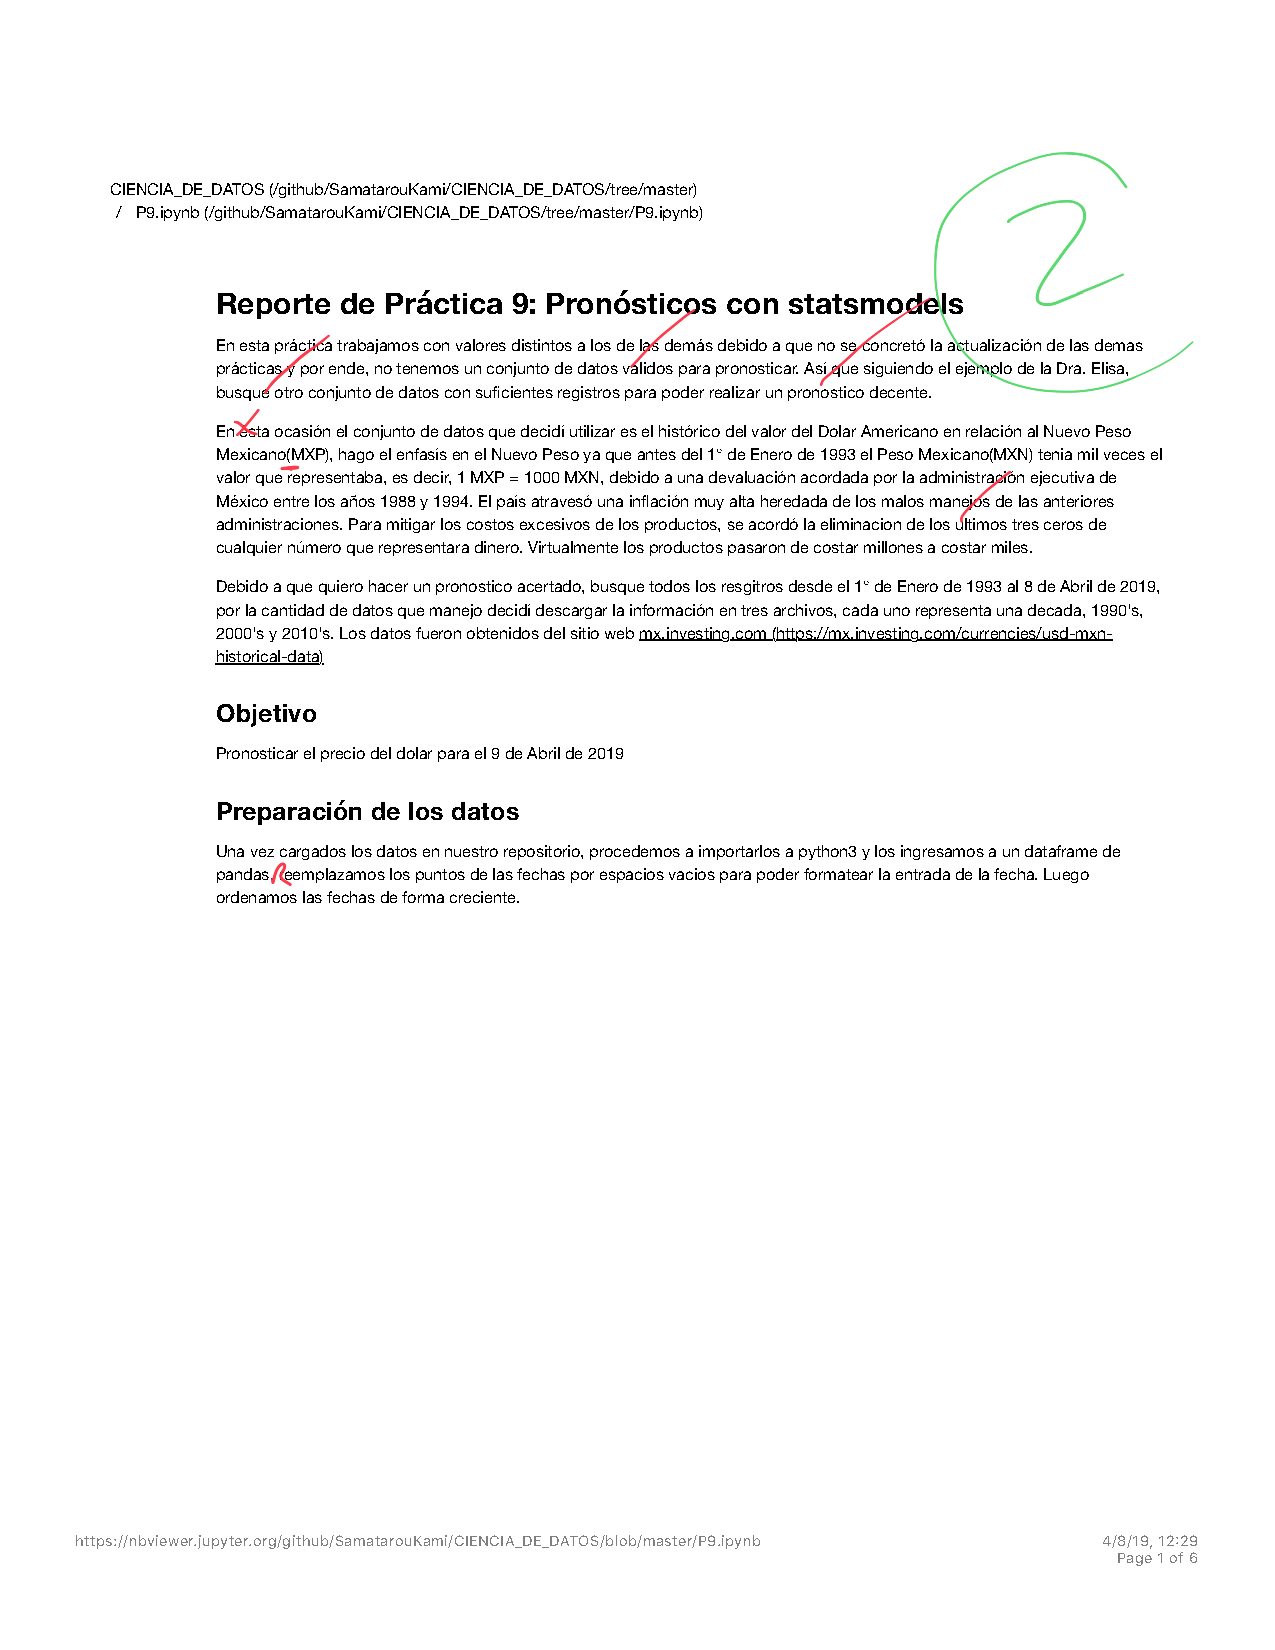
\includepdf[ pages=-, frame, scale=.85]{LA9}
\section*{Comentarios}
En esta actividad obtuve un $2/7$. La primera complicación que tuve fue con conseguir datos suficientes para poder pronosticar de la base de datos del festival de cine. Decidí buscar información en Internet de algo relevante y que tendría mercado. Busque el histórico del valor del Dólar y el peso. Obtuve 6890 días de cotizaciones, desde el 1 de enero de 1993 al 7 de abril de 2019. Mi interés era pronosticar el valor del dólar el 8 de abril. Primero me basé en el ejemplo de la Dra. Elisa, pero al no obtener buenos resultados, copie su código y empece a descomponerlo para que su funcionalidad se adaptara a mi problema. En la primera entrega fallé. Además no cumplí con el otro requisito de en base al ARIMA, conseguir los valores de $p$ y $q$ para hacer el pronóstico. En la versión mejorada logré reparar mi error, que era, variables signos especiales en el nombre. Error que también me afectó las prácticas pasadas. Por mantener la ortografía, desperdicié tiempo valioso con variables que tenían acento en su nombre.
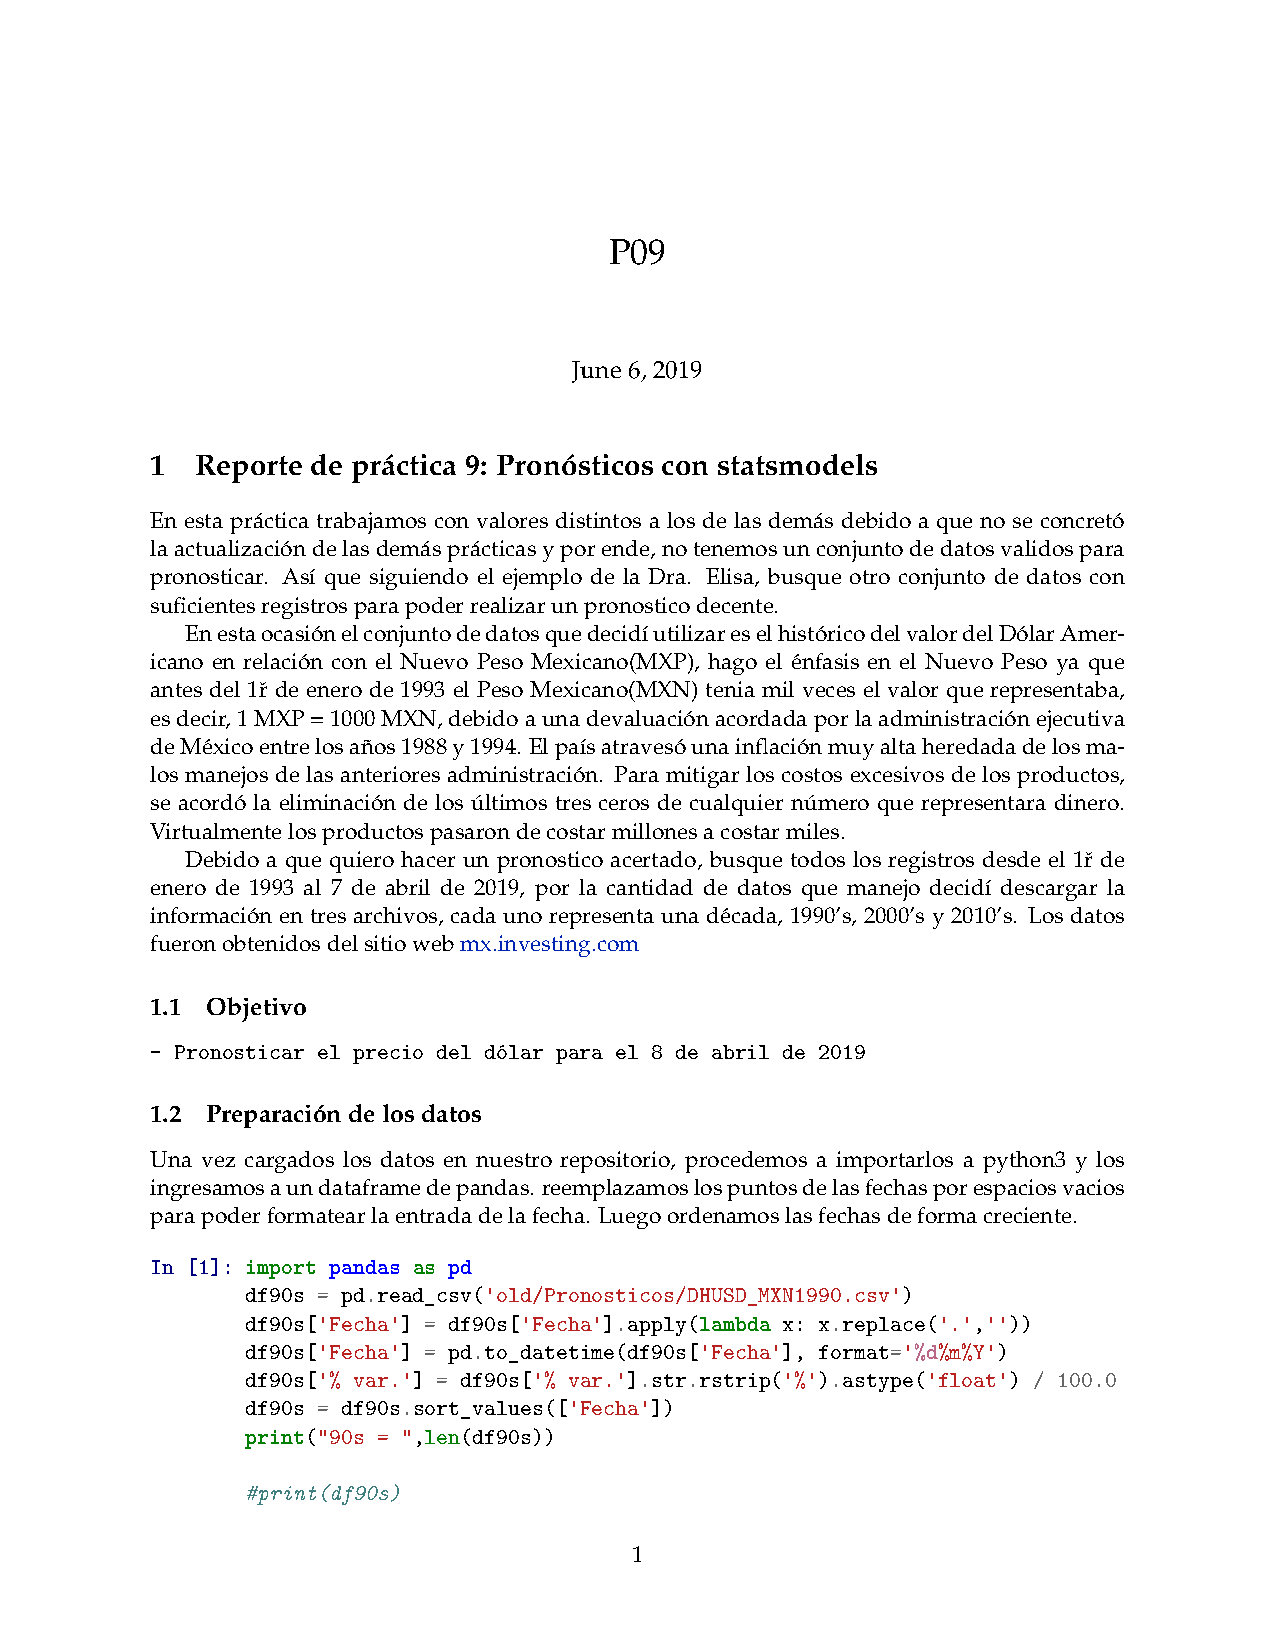
\includepdf[ pages=-, frame, scale=.85]{P09}

\chapter*{Práctica 10: Clasificación de datos}
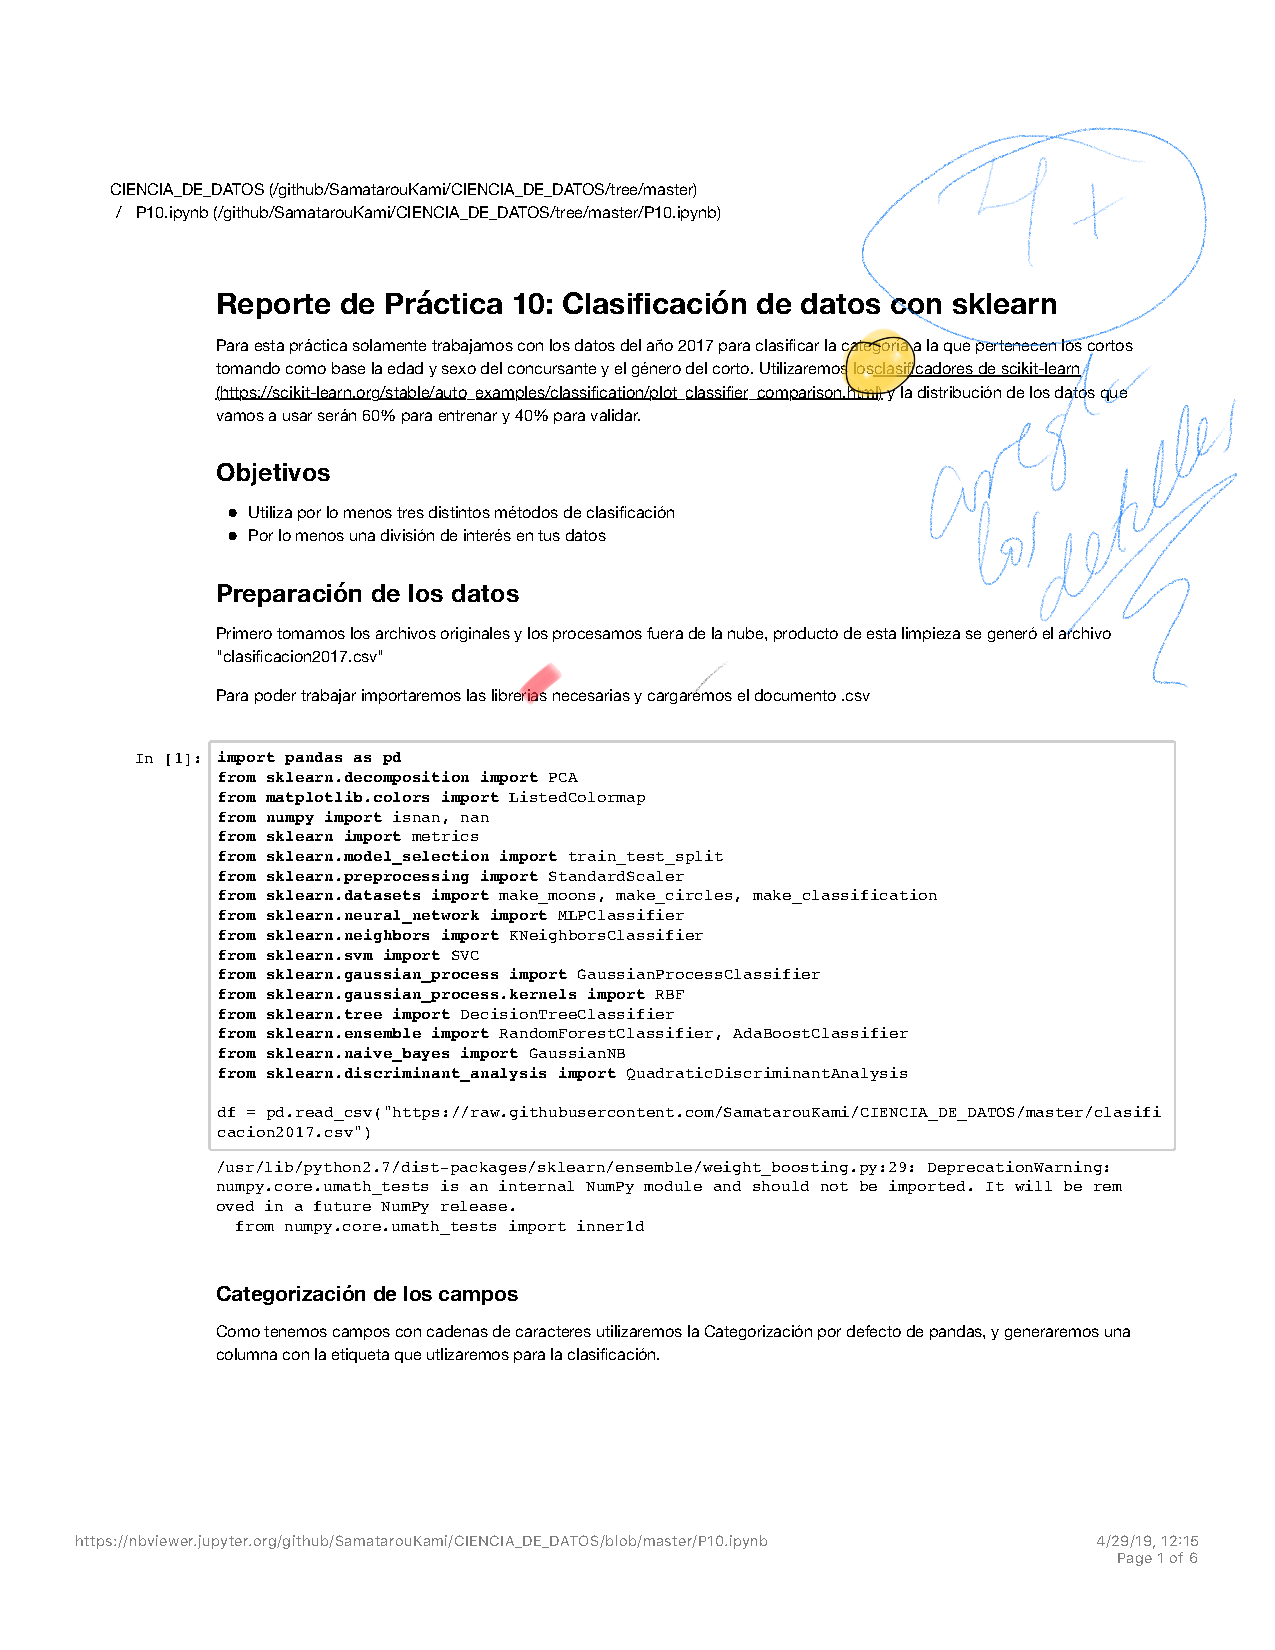
\includepdf[ pages=-, frame, scale=.85]{LA10}
\section*{Comentarios}
En esta actividad obtuve un $4/7$ debido a que aquí seguía cometiendo el error de poner las variables con signos de puntuación. En consola funcionaba bien, pero en la terminal de IPython provocaba un error. A pesar de que solo tuve errores de ortografía. También me pidieron arreglar los detalles para subir mi calificación a la hora de entregar el reporte.
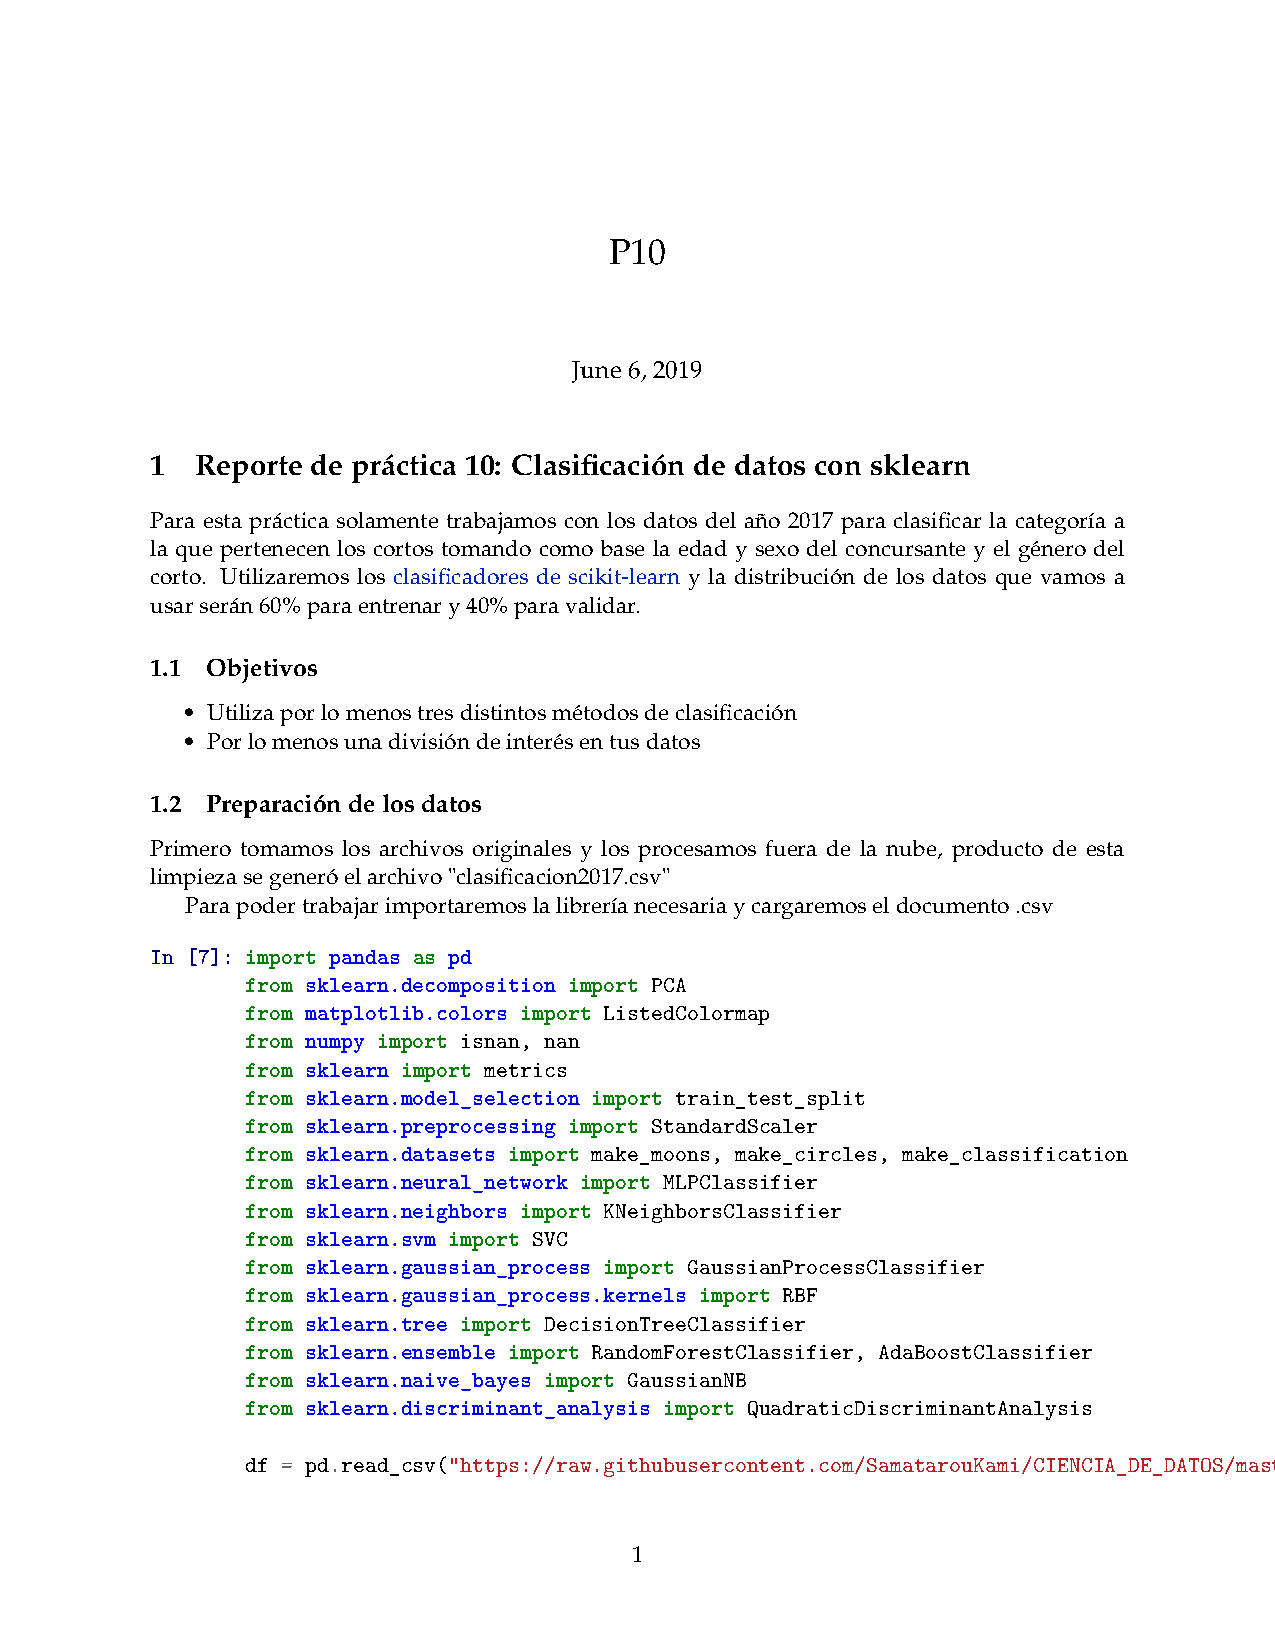
\includepdf[ pages=-, frame, scale=.85]{P10}

\chapter*{Práctica 11: Agrupamiento de datos}
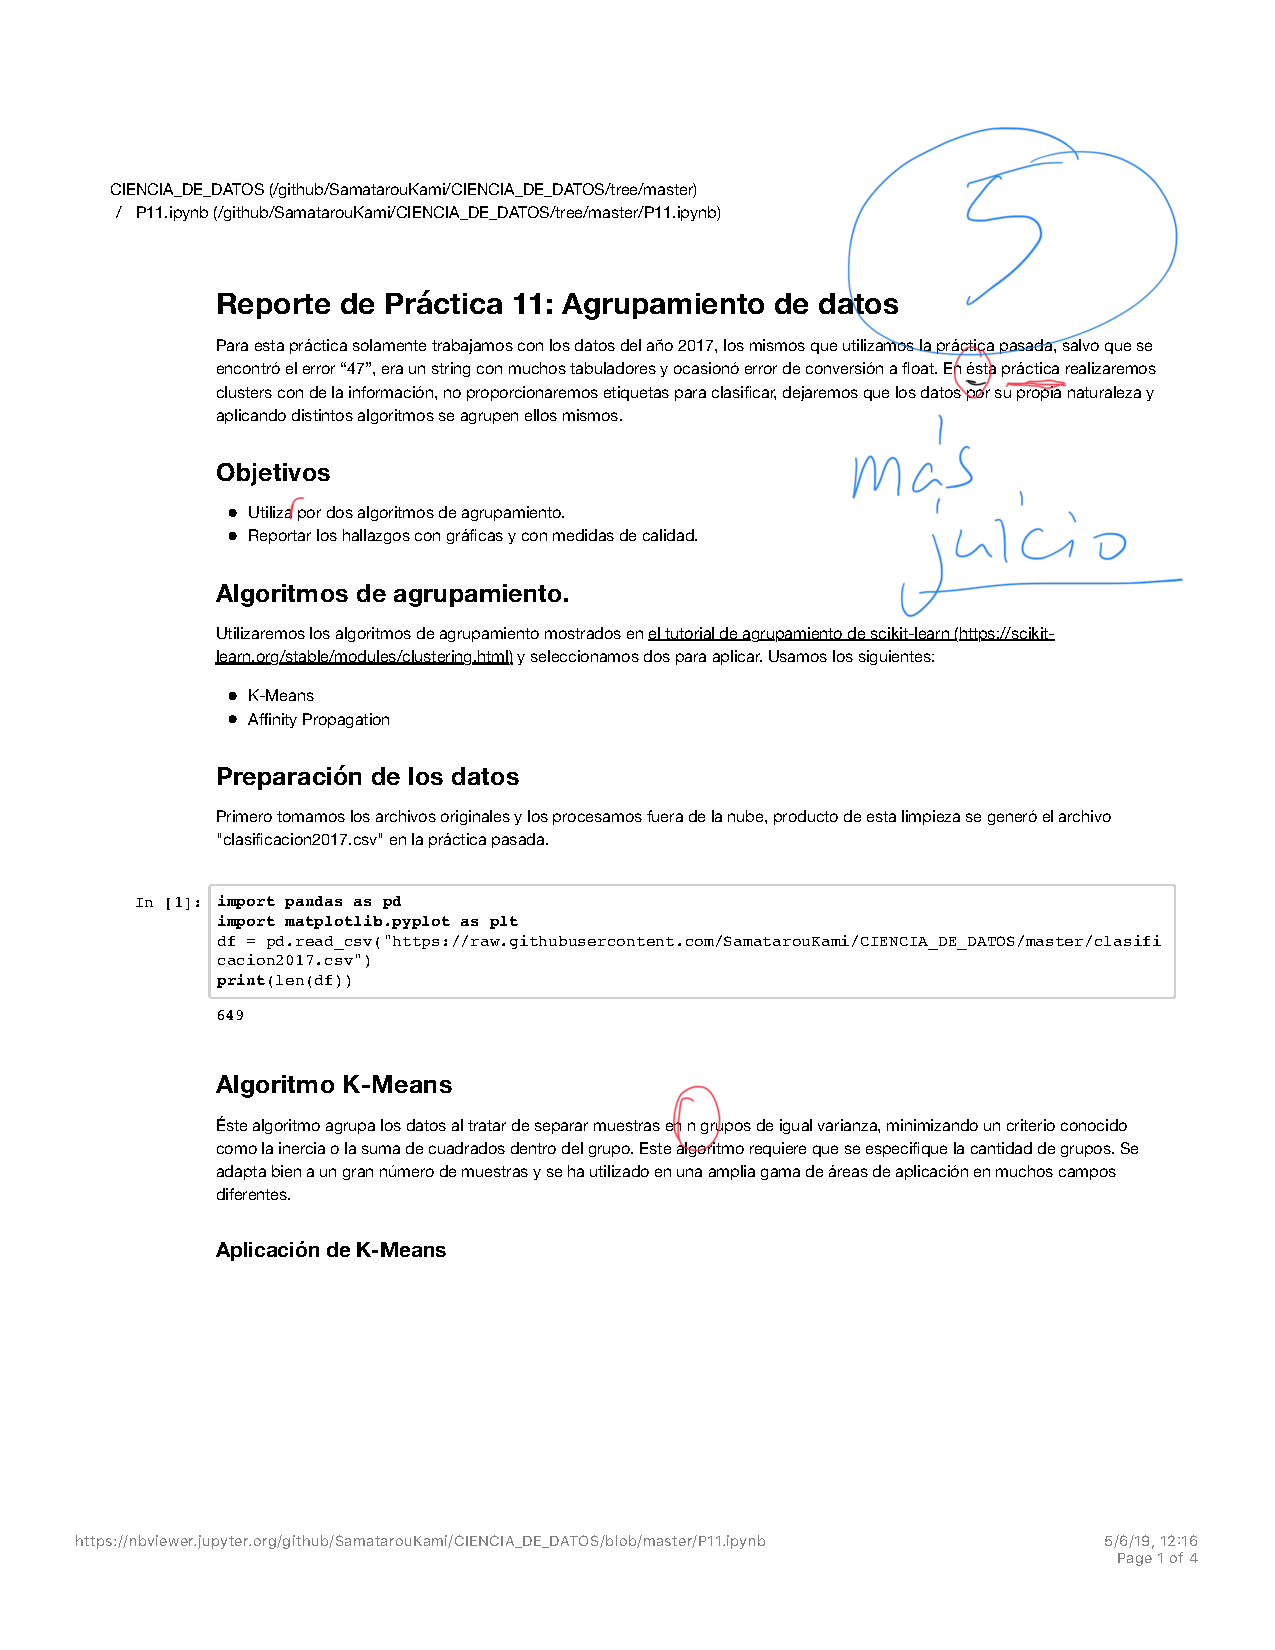
\includepdf[ pages=-, frame, scale=.85]{LA11}
\section*{Comentarios}
En esta actividad obtuve un $5/7$, hice lo que me pidieron en la tarea. La forma en la que estaban agrupados los datos usando $K$-medias no me permitieron hacer una buena agrupación. Realicé un análisis aplicando con al menos dos métodos de la librería \textit{SKLearn}, $K$-medias, y Propagación por afinidad. La Dra. Elisa me sugirió tener más criterio y buscar otro conjunto de datos que cuando usara los métodos de clasificación hubiera congruencia con la respuesta obtenida.
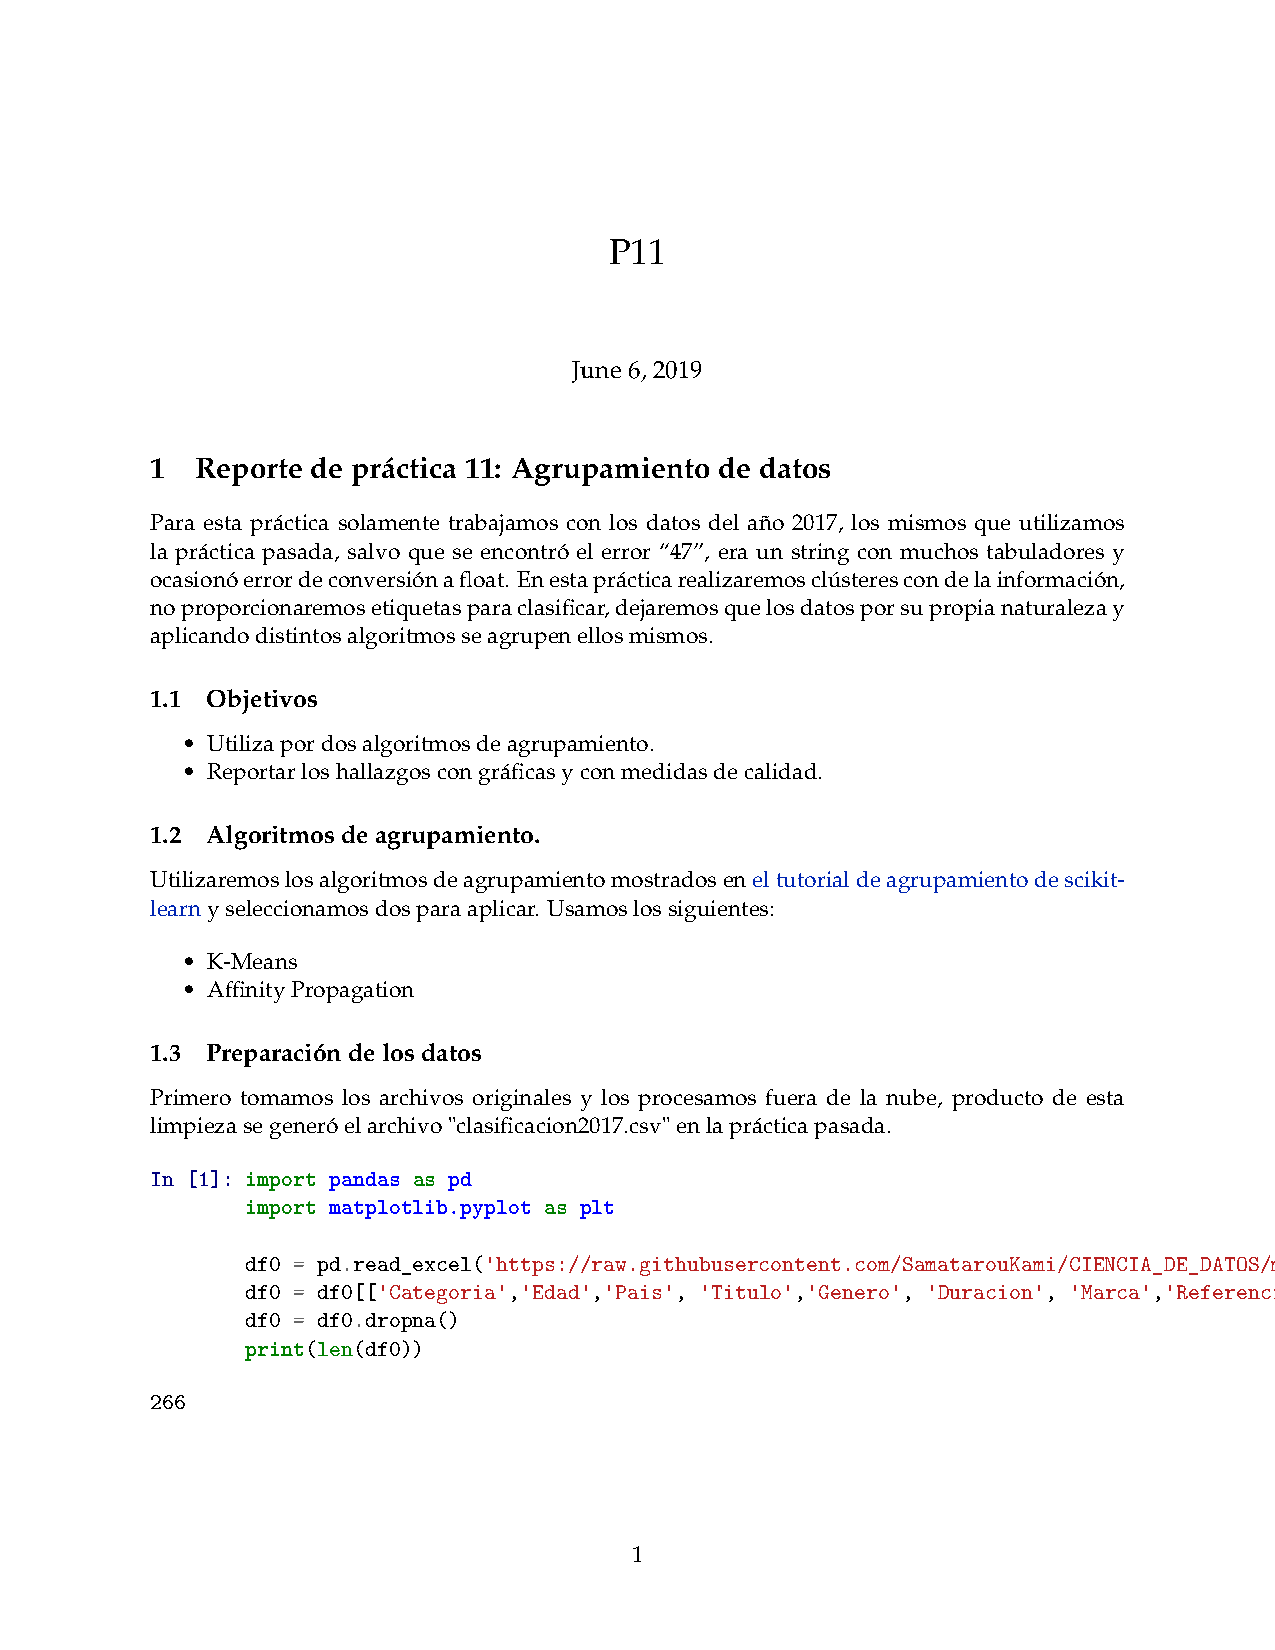
\includepdf[ pages=-, frame, scale=.85]{P11}

\chapter*{Práctica 12: Análisis de texto}
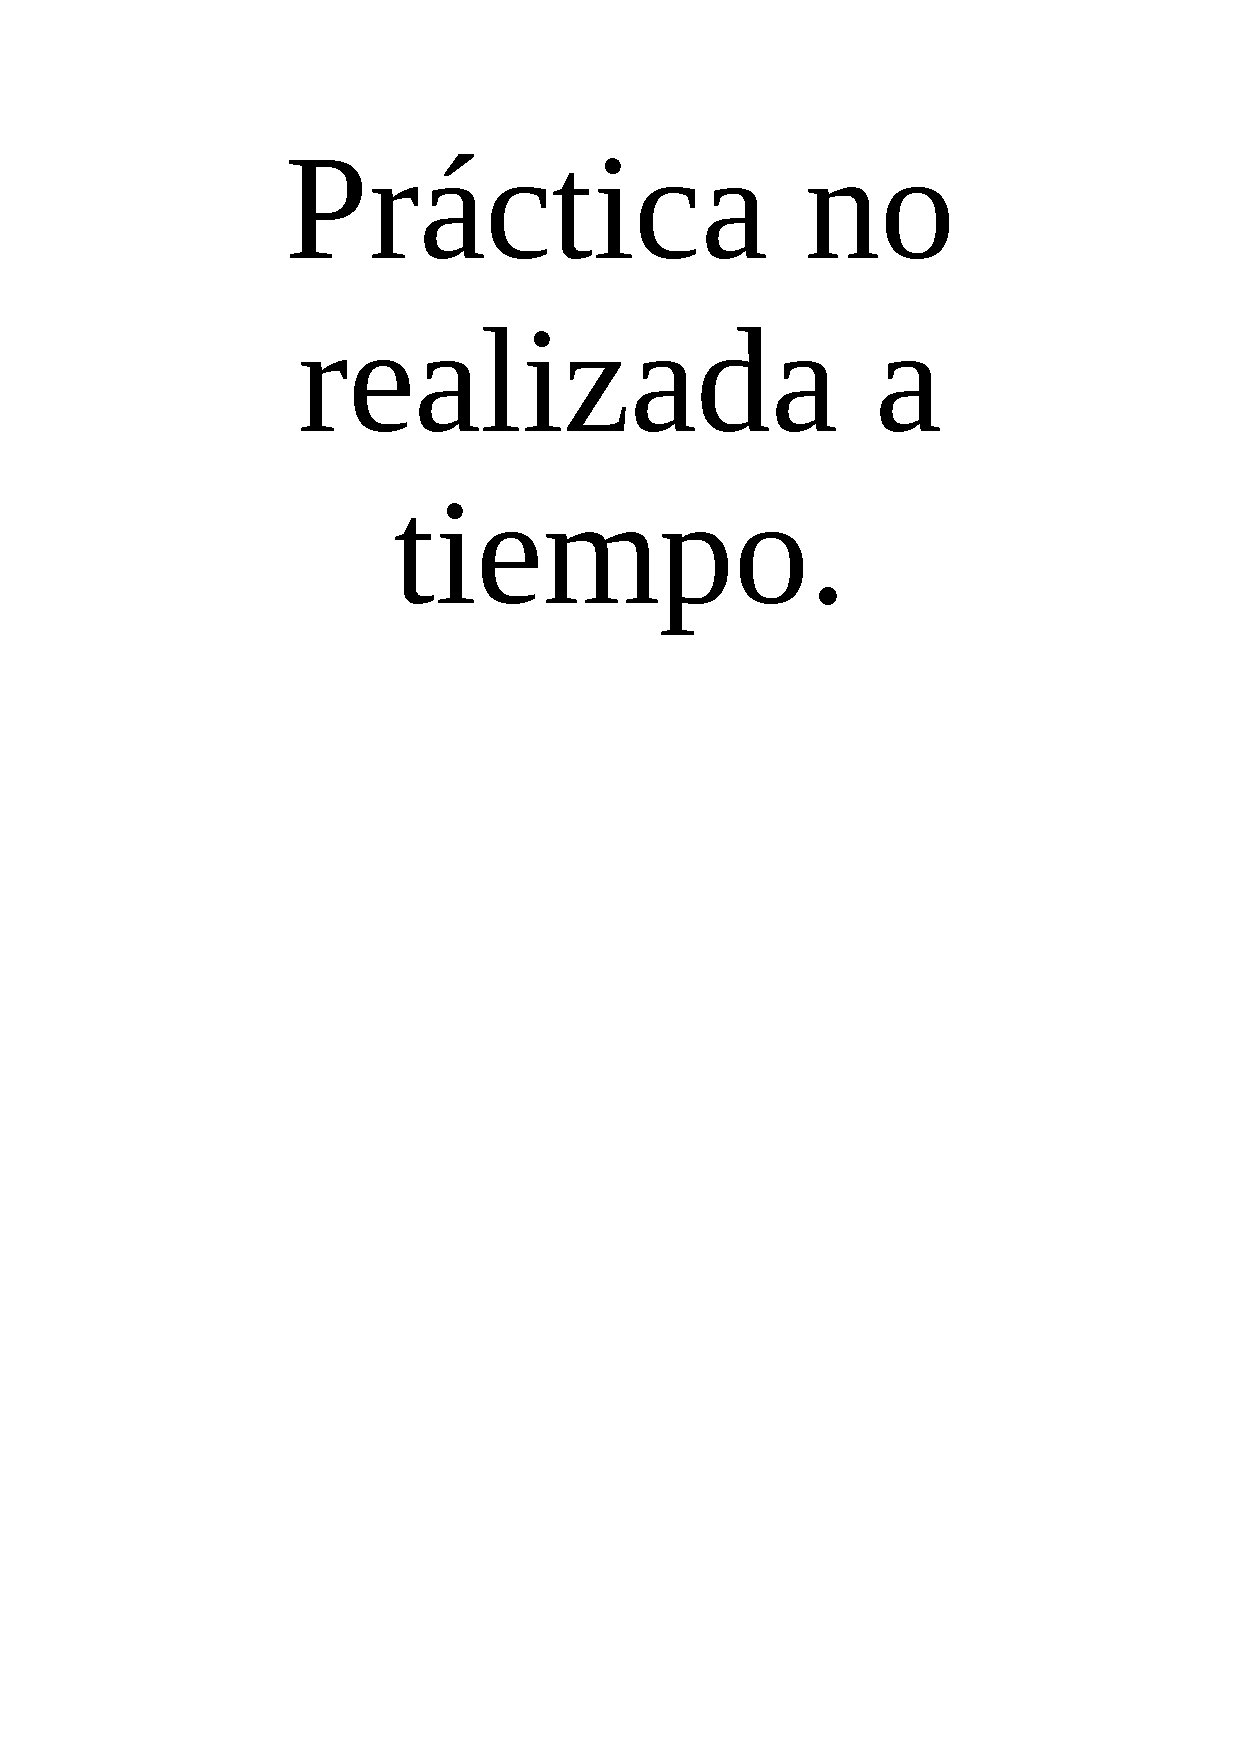
\includepdf[ pages=-, frame, scale=.85]{NP}
\section*{Comentarios}
Por no contemplar bien los tiempos de desarrollo y el tiempo de depuración de los bugs, esta tarea no pude hacerla. La preparé para entregar en este portafolio. Lo que hice fue utilizar la librería NLTK y analicé el texto de la sinopsis de los filmes.
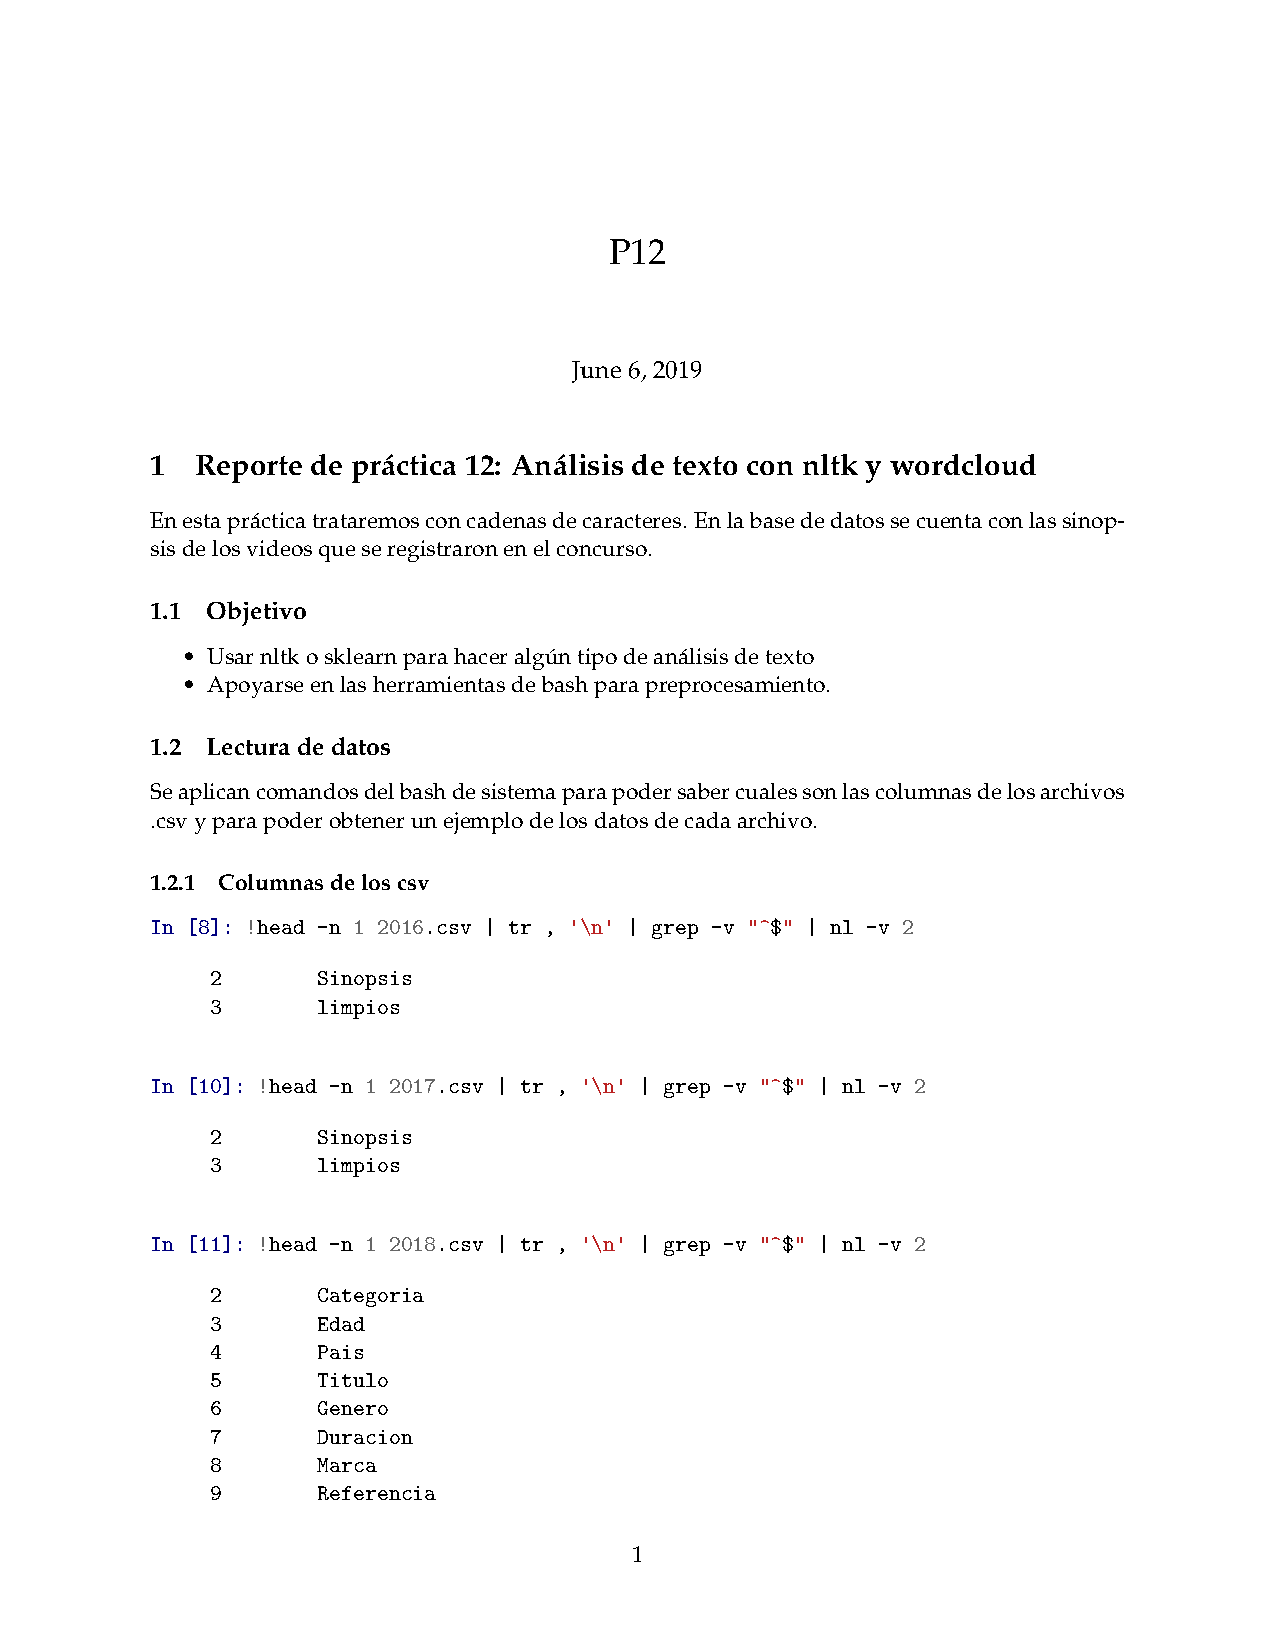
\includepdf[ pages=-, frame, scale=.85]{P12}

\chapter*{Práctica 13: Análisis de imágenes}
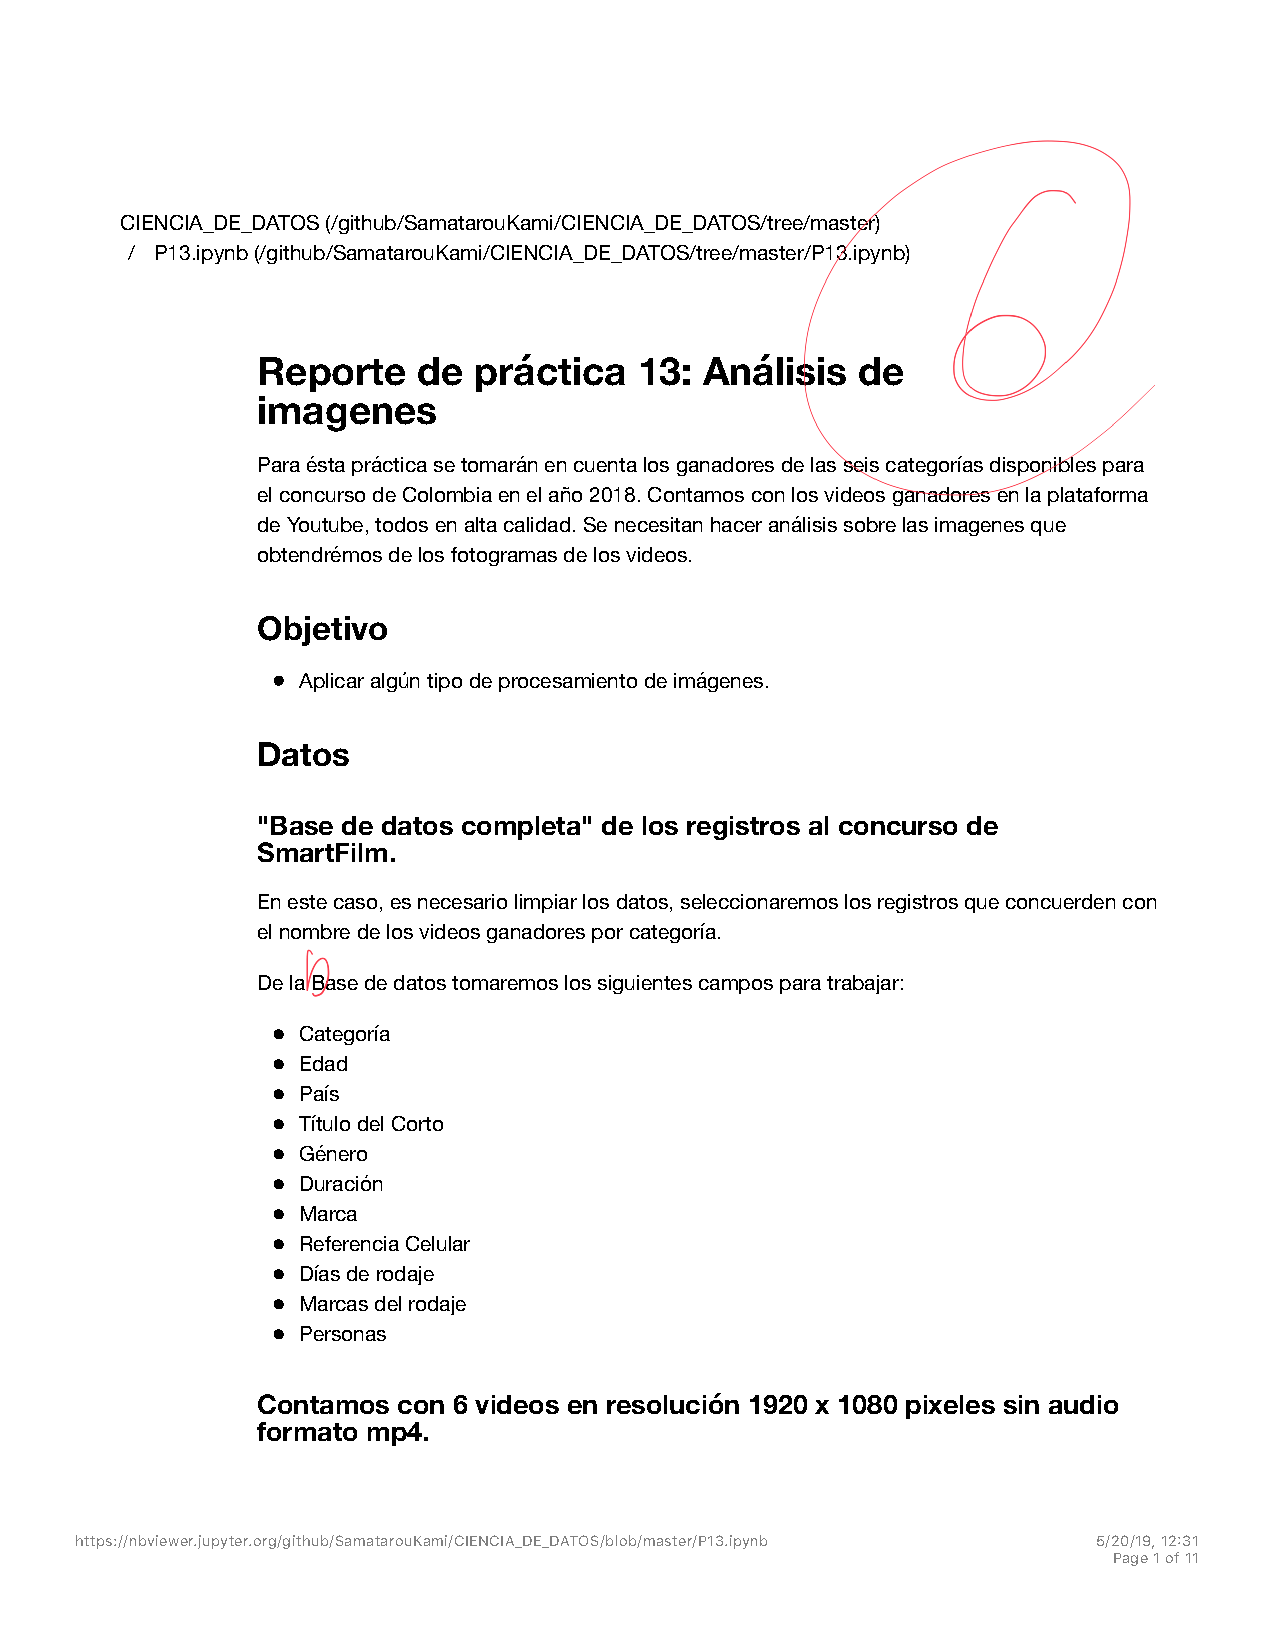
\includepdf[ pages=-, frame, scale=.85]{LA13}
\section*{Comentarios}
En esta actividad obtuve un $6/7$, cada vez mejorando, lástima que fue la ultima práctica. Tuve los errores típicos, ortografía, tiempos de conjugación verbales. Además de todo eso, dejé el proceso de saber cuantas transiciones tienen los filmes como una caja negra. En la versión corregida ya aclaro como obtuve los picos que me ayudaron a determinar las transiciones.
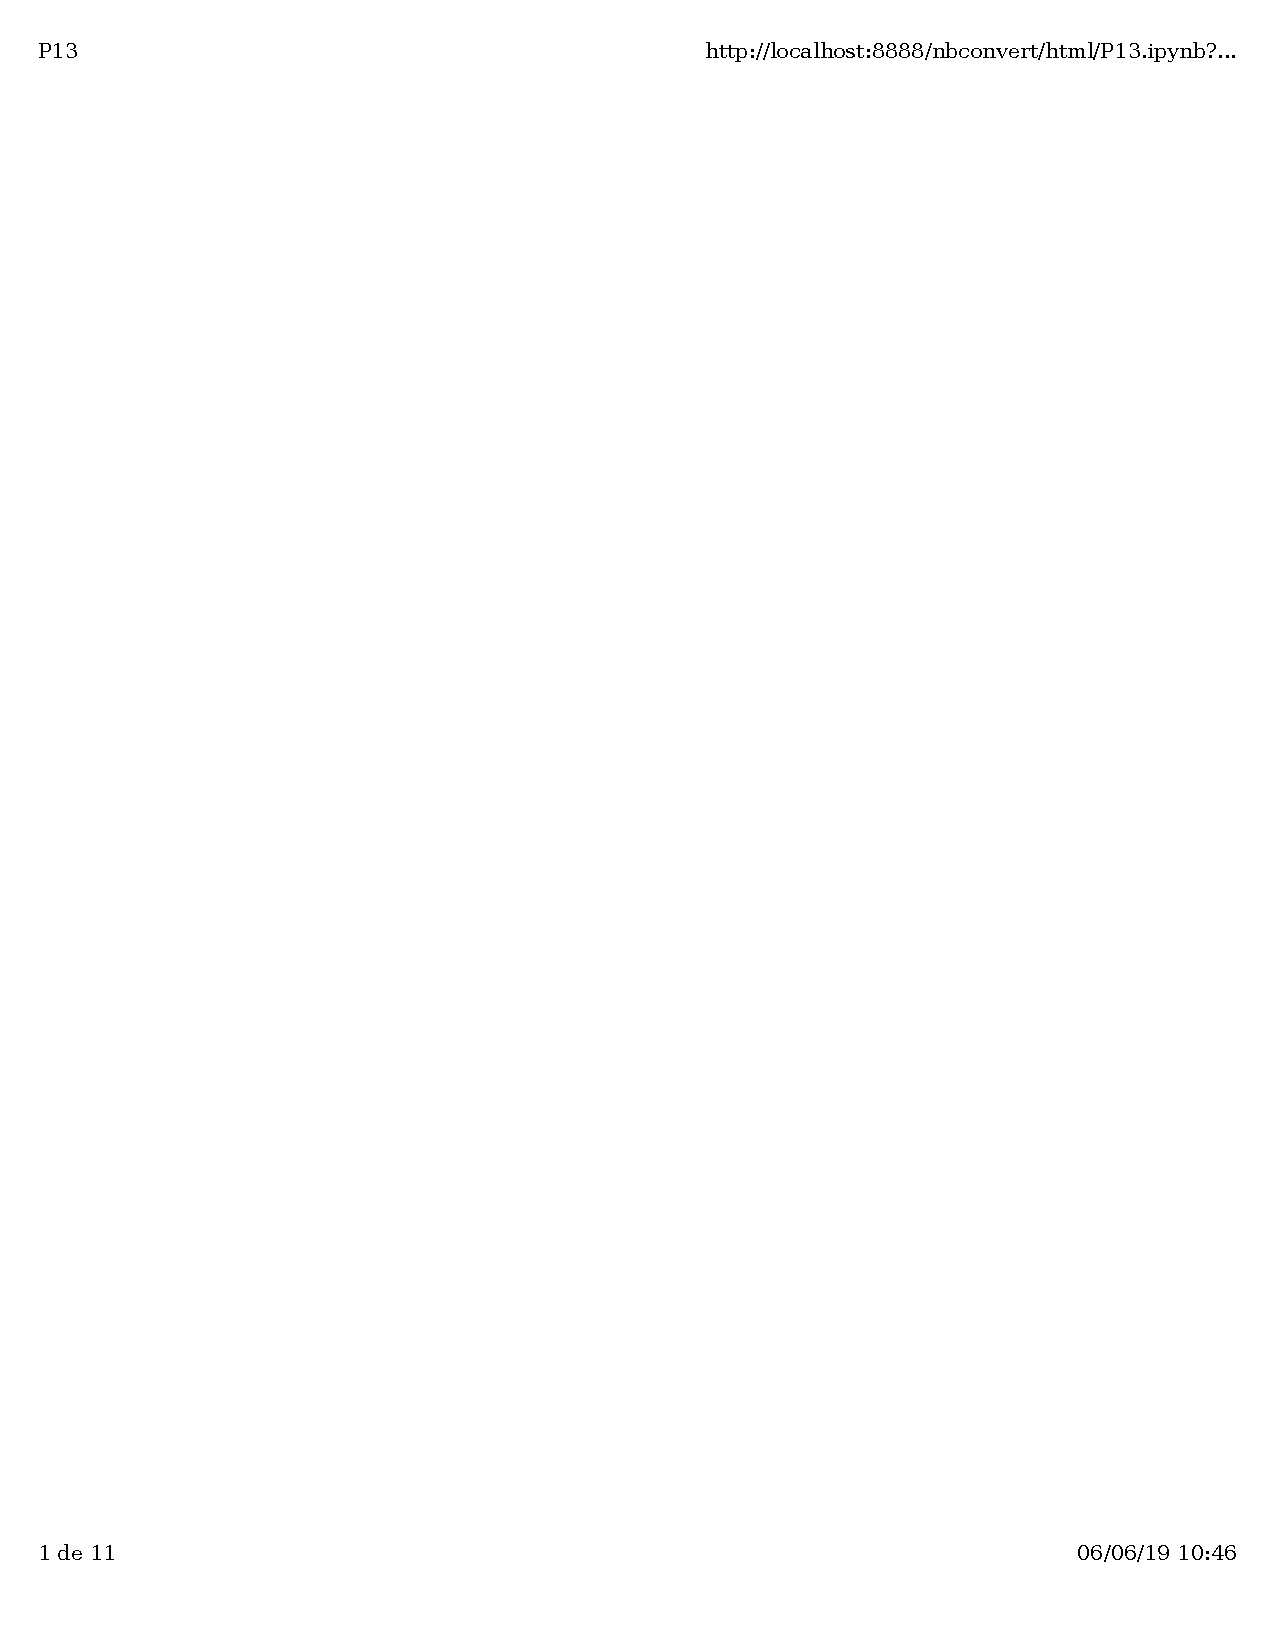
\includepdf[ pages=-, frame, scale=.85]{P13}

\chapter*{Preparación de artículo}
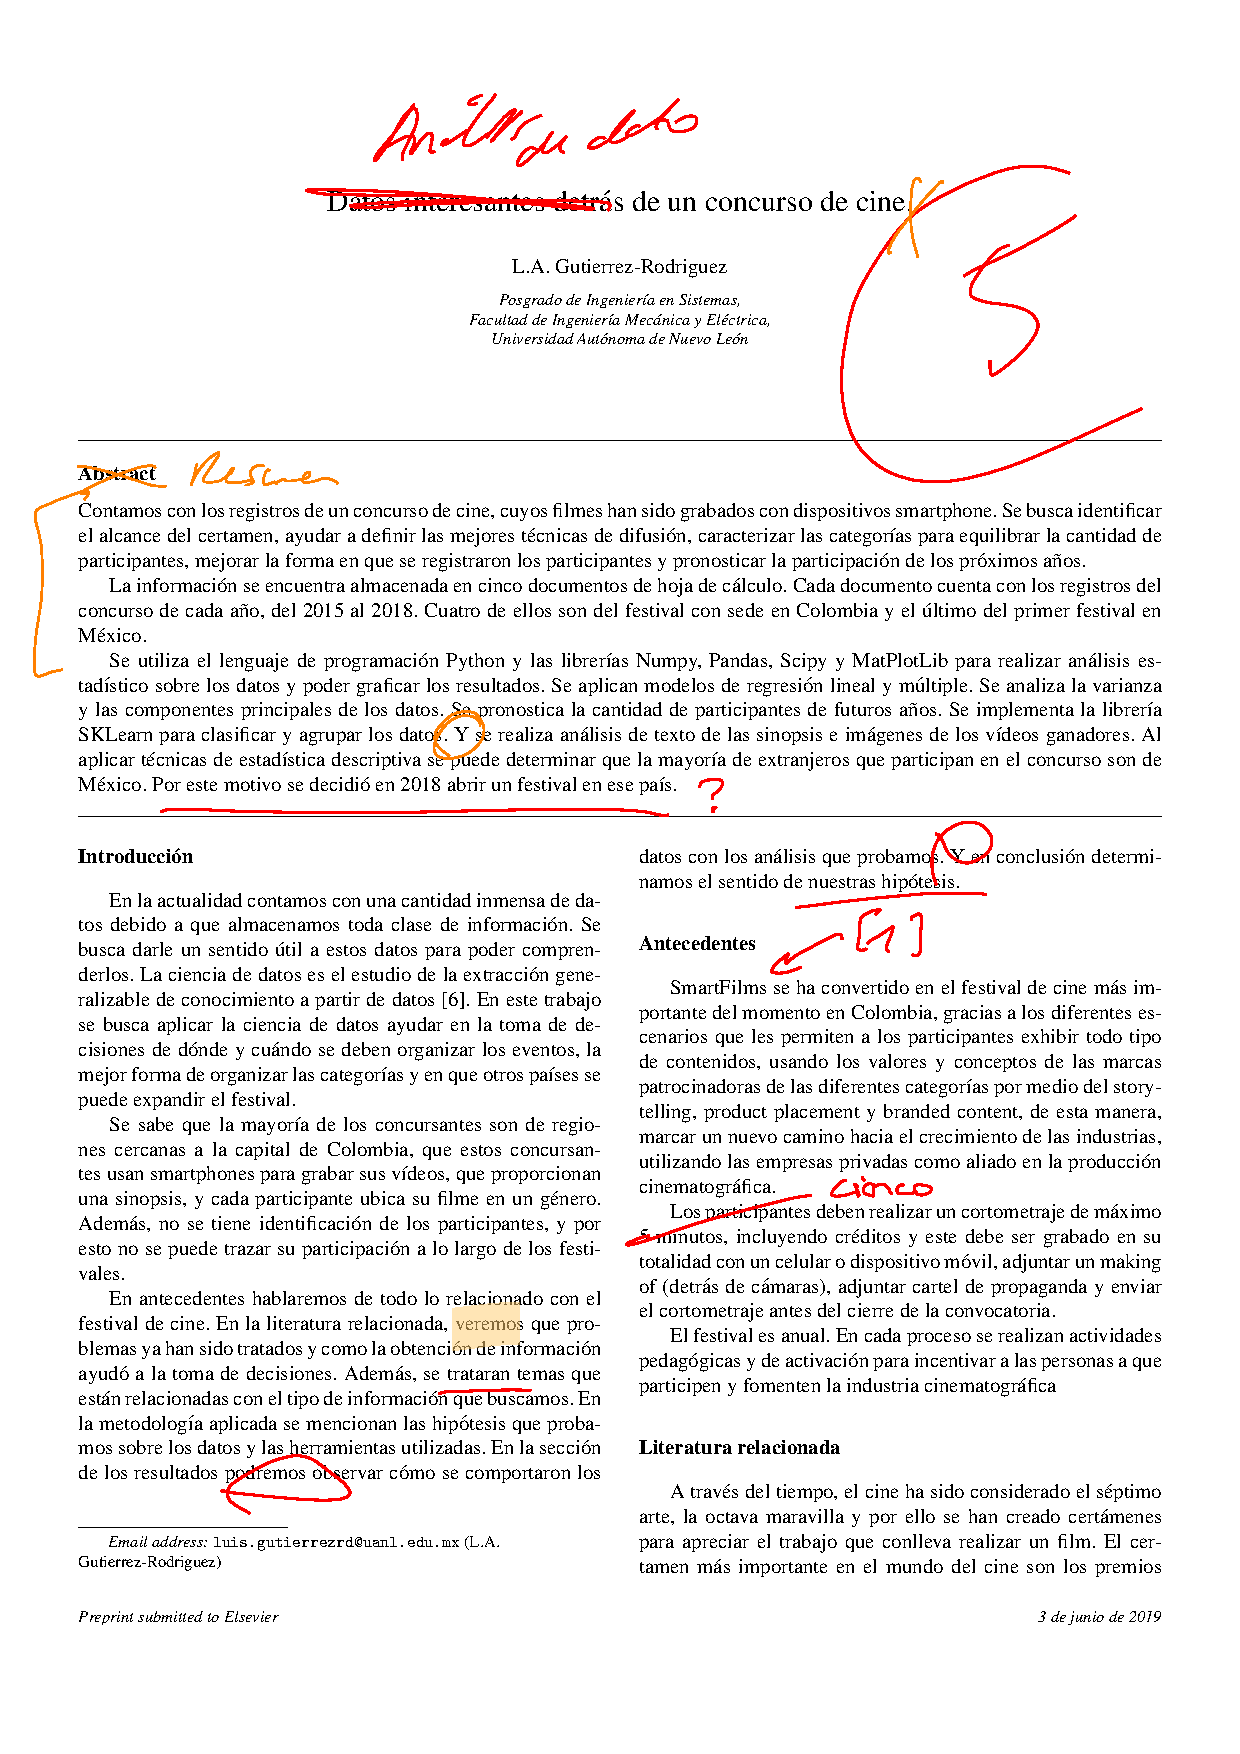
\includepdf[ pages=-, frame, scale=.85]{LAA}
\section*{Comentarios}
En el artículo cometí muchos errores, no di antecedentes de la información. No tenía gráficos congruentes con lo que quería demostrar ya que no había hecho tres prácticas a lo largo del semestre. Curiosamente las actividades múltiplos de 4, la 4, 8 y 12. Después de corregir mis prácticas, corregí el artículo, en la versión presentada en este portafolio, hice caso a las recomendaciones de la Dra. Elisa, pero además a los comentarios de las evaluaciones de mis compañeros. A mi gusto lo hice mejor que antes.
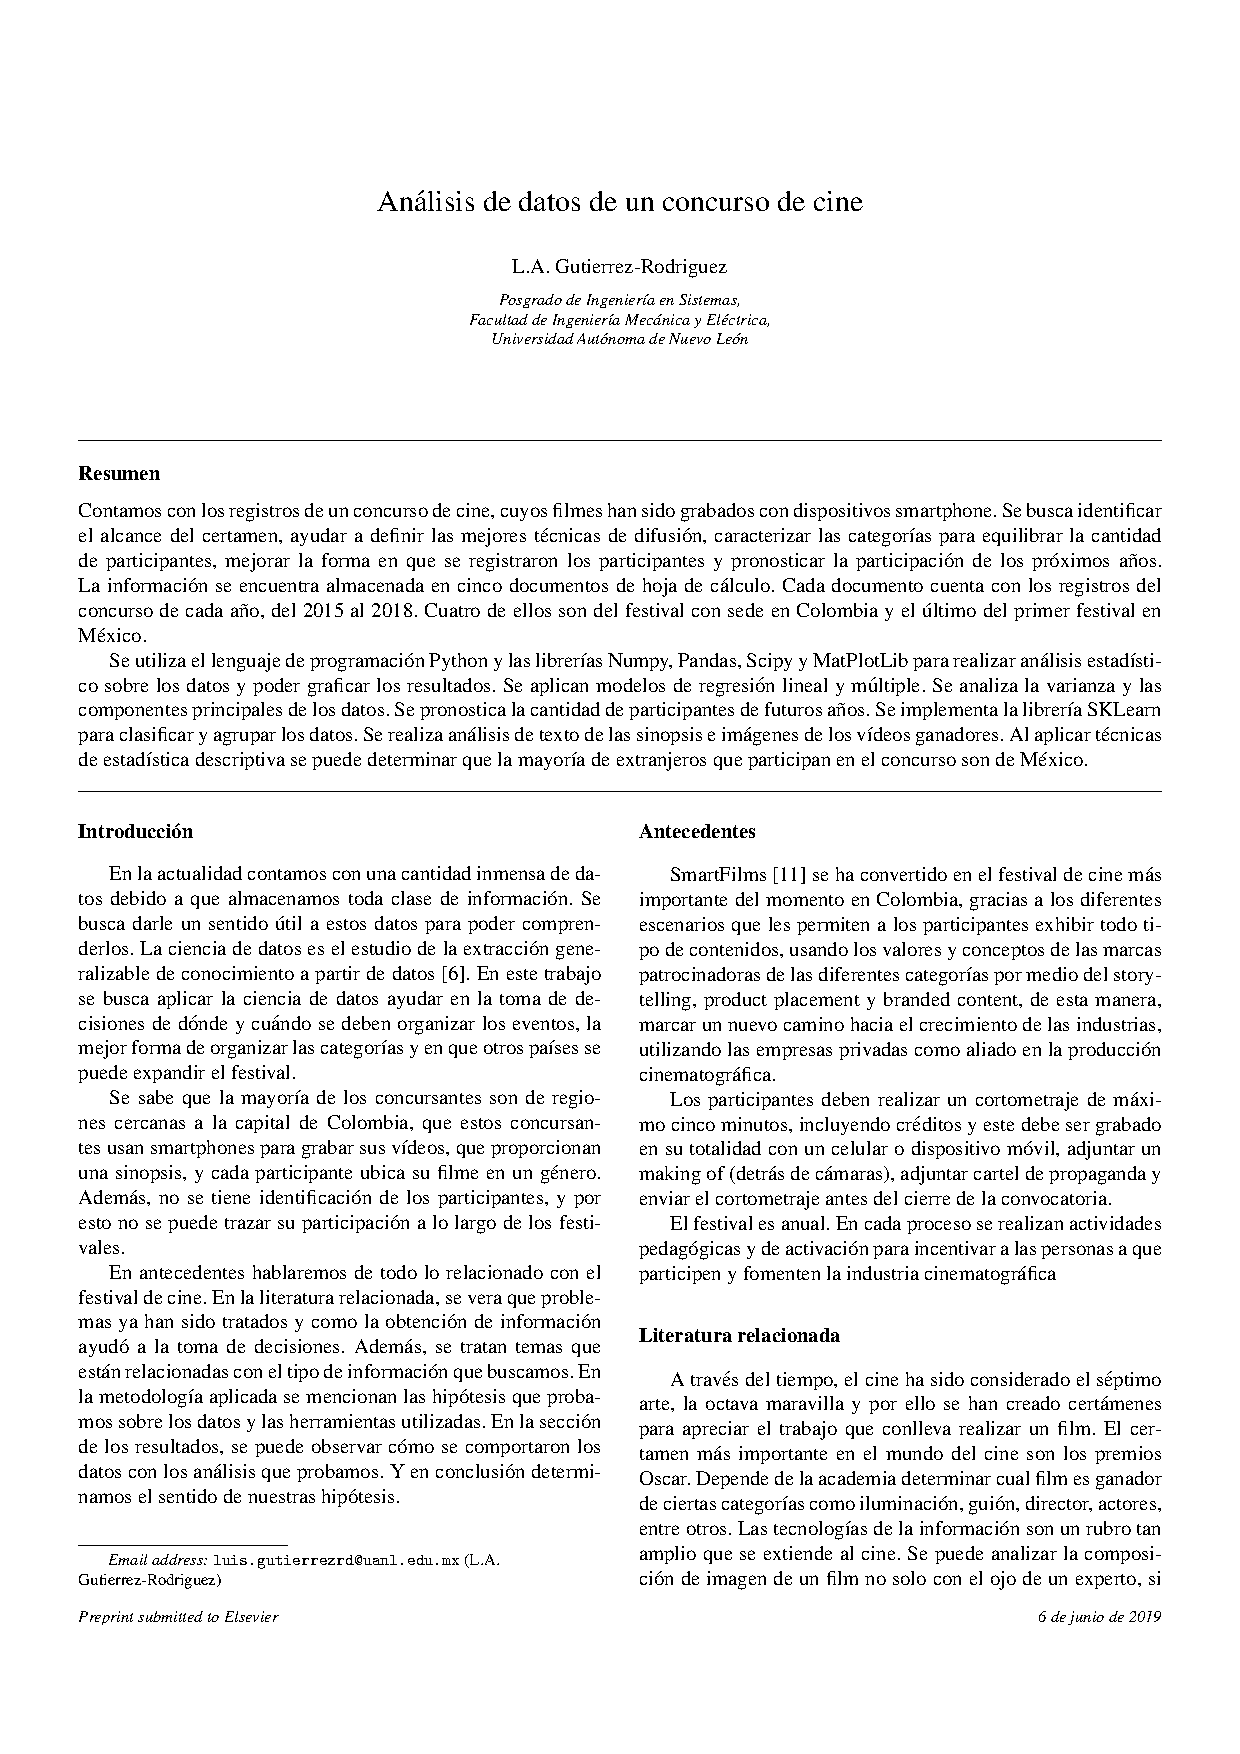
\includepdf[ pages=-, frame, scale=.85]{P14}



\end{document}